\documentclass[12pt]{article}

% Figures
\usepackage{graphicx}
\usepackage[list=true]{subcaption}
\graphicspath{{../../plots/}{../../tikz/}{../../img/}}
\usepackage[section]{placeins} % require floats to appear in the section they are defined

% fonts and appearance
\usepackage{amsmath, amsfonts, physics, siunitx}
\usepackage[american]{babel} 
\usepackage[T1]{fontenc} % improved font encoding
\usepackage[ttscale=0.8]{libertine}
\usepackage{fontawesome5}
\usepackage[format=plain, textfont=it]{caption}

% page size and margins
\usepackage{geometry}
\geometry{letterpaper,top=1in, bottom=1in, left=0.5in, right=2in}

% footer
\usepackage{fancyhdr}
\usepackage{lastpage}
\usepackage[en-US]{datetime2}
\fancyhf{}
\fancyhead[L]{CONFIDENTIAL DRAFT by J. Doss-Gollin \& K. Keller}
\fancyhead[R]{\DTMnow}
\fancyfoot[R]{page~\thepage~of~\pageref{LastPage}}
\pagestyle{fancy}

% TO DO NOTES
\usepackage{xcolor} % list of colors at https://en.wikibooks.org/wiki/LaTeX/Colors
\definecolor{giallo}{HTML}{F0BC42} % https://teamcolorcodes.com/a-s-roma-color-codes/
\definecolor{rosso}{HTML}{8E1F2F}
\definecolor{grigio}{HTML}{CACACC}
\definecolor{nero}{HTML}{000000}
\usepackage[textsize=scriptsize]{todonotes}
\setlength{\marginparwidth}{1.5in}
\newcommand{\james}[1]{\todo[color=giallo, textcolor=nero]{\textbf{ATTN James:~}#1}} % if desired create a custom command for each author
\newcommand{\klaus}[1]{\todo[color=rosso, textcolor=grigio]{\textbf{ATTN Klaus:~}#1}}

% better tables
\usepackage{booktabs}
\usepackage{array}
\newcommand{\PreserveBackslash}[1]{\let\temp=\\#1\let\\=\temp}
\newcolumntype{C}[1]{>{\PreserveBackslash\centering}p{#1}}
\newcolumntype{R}[1]{>{\PreserveBackslash\raggedleft}p{#1}}
\newcolumntype{L}[1]{>{\PreserveBackslash\raggedright}p{#1}}

% better lists
\usepackage[inline]{enumitem}
\setlist{nosep}

% authors
\usepackage{authblk}
\title{Mainstreaming Climate Adaptation Requires Subjective Integration of Deep Uncertainties}
\author[1]{James Doss-Gollin}
\author[2]{Klaus Keller}
\affil[1]{Department of Civil and Environmental Engineering, Rice University}
\affil[2]{Thayer School of Engineering, Dartmouth College}
\renewcommand*{\Affilfont}{\normalsize\normalfont}

% ACRONYMS
\usepackage[acronym,nopostdot,nonumberlist,shortcuts,]{glossaries}
\newacronym{bdt}{BDT}{Bayesian decision theory}
\newacronym{bfe}{BFE}{base flood elevation}
\newacronym[]{cdf}{CDF}{cumulative distribution function}
\newacronym{fema}{FEMA}{the Federal Emergency Management Agency}
\newacronym{gcm}{GCM}{general circulation model}
\newacronym[]{gev}{GEV}{generalized extreme value}
\newacronym{iid}{IID}{independent and identically distributed}
\newacronym{lsl}{LSL}{local mean sea level}
\newacronym{mcmc}{MCMC}{Markov Chain Monte Carlo}
\newacronym{pdf}{PDF}{probability density function}
\newacronym{rcp}{RCP}{representative concentration pathway}
\newacronym{slr}{SLR}{relative sea level rise}
\newacronym{rdm}{RDM}{robust decision making}
\newacronym[plural=SOWs,descriptionplural=states of the world]{sow}{SOW}{state of the world}
\newacronym{tc}{TC}{tropical cyclone}

\usepackage{xspace}
\makeatletter
\DeclareRobustCommand\onedot{\futurelet\@let@token\@onedot}
\def\@onedot{\ifx\@let@token.\else.\null\fi\xspace}
\def\eg{\emph{e.g}\onedot} \def\Eg{\emph{E.g}\onedot}
\def\ie{\emph{i.e}\onedot} \def\Ie{\emph{I.e}\onedot}
\def\etc{\emph{etc}\onedot} \def\vs{\emph{vs}\onedot}

\usepackage{xspace}
\makeatletter
\DeclareRobustCommand\onedot{\futurelet\@let@token\@onedot}
\def\@onedot{\ifx\@let@token.\else.\null\fi\xspace}
\newcommand{\usd}[1]{\SI{#1}[\$]{}}
\def\eg{\emph{e.g}\onedot} \def\Eg{\emph{E.g}\onedot}
\def\ie{\emph{i.e}\onedot} \def\Ie{\emph{I.e}\onedot}
\def\etc{\emph{etc}\onedot} \def\vs{\emph{vs}\onedot}

% use biblatex
\usepackage{csquotes}
\usepackage[
  backend=biber,
  doi=true,
  url=false,
  isbn=false,
  style=authoryear-comp,
  natbib=true,
  backref=false,
  maxbibnames=10,
  maxcitenames=2,
  uniquename=false,
  uniquelist=false,
  sorting=nyt,
  giveninits=true,
]{biblatex}
\renewbibmacro{in:}{}
\AtEveryBibitem{\clearfield{month}\clearfield{day}\clearfield{pages}\clearlist{language}}
\addbibresource{library.bib}

% load this last
\usepackage[hidelinks]{hyperref}
\usepackage{cleveref}

% up to 1250 words
\begin{document}
\maketitle
\thispagestyle{empty}

\begin{abstract}
    \textbf{Draft in preparation to Earth's Future}.
\end{abstract}

\clearpage

\section{Introduction}\label{sec:introduction}

Since infrastructure built today is likely to persist for several decades, infrastructure designs must take into account the stresses that a project is likely to face decades into the future.
On the one hand, overly optimistic assumptions of future risk can lead to unacceptably high risk of failure in the future if additional investments are not made.
For example, a failure to prepare Texas's interconnected natural gas, electricity, and water systems for temperatures that had been observed in the past 30 years caused cascading failures with disparate impacts \citep{doss-gollin_txtreme:2021,busby_cascadingrisks:2021}.\james{Too fast on intro. Need to slow down and define concepts}
On the other, unless opportunity costs are negligible, designing for a too-pessimistic scenario can contribute to maladptation by limiting resource availability in the future.
For example, \ldots\james{add an example of a maladaptive megaproject -- look to sustainability science or the arguments in \citet{ansar_bigisfragile:2017}, something by Flyvbjerg, \etc}

TODO: set up flood risk management as a context where over- or under-design could be relevant, then raise house elevation in the coastal zone as a specific example.
Federal guidance for this decision relies on standards (the $T$-year flood) rather than risk-based design.
Be sure to note that this has parallels to lots of other engineering design guidance. Then note the work of \citet{zarekarizi_suboptimal:2020} or \citet{xian_elevation:2017}, who show that a risk-based approach may improve considerably on a standards-based approach.

Additionally, the floodplain maps used for decision supportare silent on projected future changes and neglect the deep and dynamic uncertainties surrounding the projected hazards\ldots
Both risk-based design and standards-based approaches are complicated by nonstationarity.
On the one hand, nonstationarity of flood hazard is already evident in many places, especially in coastal areas where \gls{slr} is clear.
On the other, efforts to find objective methods for quantifying nonstationarity, eg of precipitation \citep{atlas14_texas:2018} or flood frequency \citep{bulletin17c:2019}, have struggled to find a satisfactory approach because factors like future emissions and localized climate response create deep uncertainties that resist objective quantification \citep[\eg,][]{keller_management:2021}.

This motivates subjective approaches for designing for nonstationarity.
Thus decision-makers need some subjective way to choose which possible futures to design for.

In this paper, we use a didactic case study of house elevation in Norfolk, VA as a lens through which to shed light on the following research questions.
\begin{description}
    \item[Q1] What are the potential benefits to homeowners of changing threshold-based guidance to risk-based guidance under nonstationary flood hazard?
    \item[Q2] How does risk-based guidance change under different assumptions of physical model structure and human emissions forcings?
    \item[Q3] How can deep uncertainties be transparently and consistently synthesized for decision analysis?
\end{description}
Specifically, we examine this problem through three lenses.\james{Which ones?}

The paper is organized as follows.\james{This is confusing to the reader}
In \cref{sec:case-study} we describe our case study in Norfolk, VA.
First, in \cref{sec:multiple-simulation} we analyze each simulation (\ie, realizations from these \glspl{pdf}) independently and illustrate .
Next, in \cref{sec:multiple-pdf} we consider the design problem as a set of ``multiple \glspl{pdf}'' and use these findings to motivate theoretical advances.
Then in \cref{sec:synthesizing} we present a probabilistic method for synthesizing simulations from multiple \glspl{pdf} and illustrate the advantages and potential pitfalls of this approach.
Finally in \cref{sec:conclusions} we briefly summarize our findings, discuss implications for engineering practice, and identify  future research needs.

\section{Case study}\label{sec:case-study}

We model a \emph{hypothetical} house in Norfolk, VA, where sea level rise drives nonstationary future flood hazard.
For interpretability, we focus on deep uncertainty in \gls{slr} and treat other model parameters as fixed quantities or as outputs from a single probabilsitic model, as shown in \cref{tab:uncertainties}.
We consider a single, one-time decision of whether to elevate a house, and if so by how much (\cref{fig:xlrm}).
We evaluate this decision for each of many possible simulations of \gls{slr} using a combined engineering-economic model based on that of \citet{zarekarizi_suboptimal:2020}.
In the remainder of this section we discuss data sources and the system model.

\begin{table}
    \centering
    \caption{Summary of uncertainties modeled and their treatment.}\label{tab:uncertainties}
    \begin{tabular}{l l p{3in} l}
        \toprule
        Name             & Symbol           & Conceptual framework                                                                 & Section               \\
        \midrule
        \Gls{slr}        & $\overline{y}_t$ & Deeply uncertain: multiple methods considered                                        & \ref{sec:sea-level}   \\
        Storm surge      & $y'_t$           & Probabilistic: a single stationary \acrshort{gev} model                              & \ref{sec:storm-surge} \\
        Discount rate    & $1-\gamma$       & Fixed at 3\%                                                                         & \ref{sec:ead}         \\
        Depth-damage     & $D(h-y_t)$       & Deterministic: based on HAZUS model                                                  & \ref{sec:ead}         \\
        Elevation cost   & $C(\Delta h)$    & Deterministic: a piecewise linear model following \citet{zarekarizi_suboptimal:2020} & \ref{sec:sow-metrics} \\
        Initial height   & $h_0$            & Deterministic: \SI{1}{ft} below the \gls{bfe} unless otherwise noted                 & TBD                   \\
        House floor area &                  & Deterministic: \SI{1500}{ft^2} unless otherwise noted                                & TBD                   \\
        Structural value &                  & Deterministic: \usd{200000} unless otherwise noted                                   & TBD                   \\
        House lifetime   &                  & Deterministic: 70 years unless otherwise noted                                       & TBD                   \\
        \bottomrule
    \end{tabular}
\end{table}

\begin{figure}
    \centering
    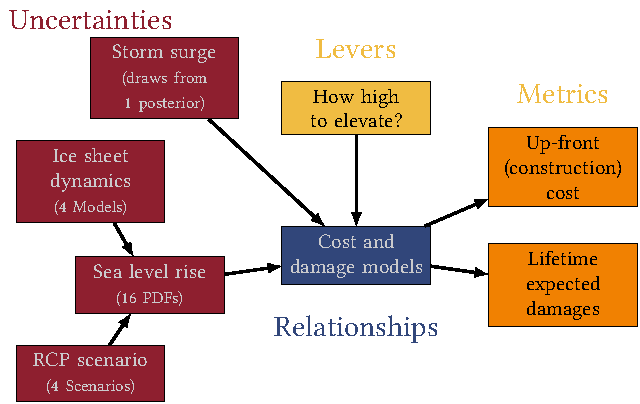
\includegraphics[width=4in]{xlrm.pdf}
    \caption{
        Conceptual diagram of the decision problem.
        A \gls{sow} consists of a description of the uncertain factors (red).
        We model a single decision (yellow).
        For each combination of \gls{sow} and policy, the system model (gray) is used to calculate metrics describing the performance of the policy over the selected \gls{sow}.
    }\label{fig:xlrm}
\end{figure}

\subsection{Sea level rise}\label{sec:sea-level}

Deeply uncertain sea level rise is the focus of our model.
Our analysis considers the common case where a decision maker or analyst has access to an existing set of simulations.
Specifically, we use simulations published in \citet{ruckart_hazardous:2008} that use the BRICK model version 0.2 \citep{wong_brick0.2:2017}.

\Cref{fig:msl-boxplots} shows the \glspl{pdf} of mean sea level in 2100 under each of the eight models considered: four emissions pathways \citep[\gls{rcp} scenarios][]{moss_rcp:2010} and two models of ice sheet dynamics.
Variation between different \glspl{pdf} is dominated by the \gls{rcp} 8.5 scenario with fast ice sheet dynamics \citep[see][for a discussion of these dynamics]{wong_brick0.2:2017}.
This is also the \gls{pdf} with the greatest within-model variance.
\begin{figure}
    \centering
    %\includegraphics[width=5in]{msl_boxplots.pdf}
    \caption{
        Sea level rise projections use the BRICK model \citep{wong_brick0.2:2017,ruckert_coastal:2019}.
        We consider \emph{eight time-dependent PDFs of sea level rise}: four \gls{rcp} scenarios $\times$ two parameterizations of ice sheet processes.
    }\label{fig:msl-boxplots}
\end{figure}

For consistency with previous studies, we refer to one time series of \gls{slr} ($\overline{y}_t$) as \emph{a \acrfull{sow}}.

\subsection{Storm surges}\label{sec:storm-surge}

Neglecting hydrodynamics, we model annual maximum floods $y_t$ as the sum of sea level $\overline{y}_t$ and storm surges $y'_t$.

Data on storm surge comes from Sewells Point, VA (NOAA gauge 8638610).\james{cite NOAA data source}
Hourly recordings of water level are available from 1928 to the present; we use data from the period January 01 1928 to December 31 2021.
For each year we remove the annual mean then extract a single maximum; we refer the set of these maxima for all years as the time series of annual maximum storm surges.
This time series is shown in \cref{fig:observed-surges}(a).
In (b) we use the Weibull plotting position
\begin{equation}\label{eq:plot-pos}
    \frac{r}{N + 1}
\end{equation}
where $N$ is the sample size and $r$ is the order of the $N$ observations ($r=1$ is the largest, $r=N$ is the smallest).

\begin{figure}
    \centering
    %\includegraphics[height=1.5in]{historic_surge.pdf}%
    %\includegraphics[height=1.5in]{surge_return_period.png}
    \caption{
        Annual maximum storm surges (after subtracting mean sea level) at Sewells Point, VA (CITE SOURCE).
        (a):
        Time series of historic storms.
        Purple (orange) arrows denote notable tropical cyclones (nor'easters).
        (b):
        Return periods.
        Dots indicate observed values; their $x$-value (``plotting position'') is calculated using the Weibull formula (eq.~\cref{eq:plot-pos}).
        Blue line shows a maximum likelihood \gls{gev} fit and the gray lines show Monte Carlo draws from the full posterior distribution of the Bayesian GEV fit.
    }
    \label{fig:observed-surges}
\end{figure}

We model future storm surge risk through a probabilistic lens.
To do this, we develop a stationary\james{discuss / validate this -- it's cool, we have the supplemental info and can emphpasize our focus here is on SLR for didactic purposes} Bayesian model for storm surge:
\begin{equation}\label{eq:surge-model}
    y'_t \sim \text{GEV}\left(\mu, \sigma, \xi \right),
\end{equation}
where $y'_t$ is the storm surge (above sea level) in year $t$ and $\mu$, $\sigma$, and $\xi$ are the location, scale, and shape parameters, respectively.

When \gls{gev} distributions are fit to time series data without strong prior information, the resulting uncertainties can be unrealistically large.\james{cite}
Thus, information from other locations, time periods, and/or from physical principles may help to reduce uncertainties \citep{Merz:2008bl,Merz:2008eh}.
To constrain estimates, we add weakly informative priors.
However, rather than adding prior information over the parameters themselves, we follow \citet{coles_evd:1996} and apply a prior over extreme quantiles of the distribution.
Specifically, we apply LogNormal priors over the 90th, 99th, and 99.9th percentiles of the distribution (\ie, the 10, 100, and 1000 year return period events).\james{Expand on this ``probabilistic inversion''}
These values were chosen to represent plausible physical ranges (the assumed 90\% confidence interval for the 10 year event is XY years, for the 100 year event is XZ years, and for the 1000 year event ZY years) and are plotted in supporting figure SX.\james{return to this sentence}

To evaluate a single \gls{sow}, we integrate over $J$ samples from the posterior distribution (of \cref{eq:surge-model}).

\subsection{Expected annual damage}\label{sec:ead}

There are two components of the system model (``relationships'' in \cref{fig:xlrm}).
The first is a fragility model that estimates the expected flood loss for a particular year, given the elevation of the house and the mean sea level for that year.
Specifically, expected annual damages in year $t$ is defined as the expected damages in a given year, conditional on the house's height relative to the gauge after elevation ($h = h_0 + \Delta h$):
\begin{equation}
    \textrm{EAD}_t = \mathbb{E}[d_t | h] = \int_{y_t} p(y_t) D(h - y_t) dy_t,
\end{equation}
where $y_t = \overline{y}_t + y'_t$ is the annual maximum flood, relative to the gauge, in year $t$, and $D(h - y_t)$ is the damage as a function of depth relative to the house.
Following \citet{zarekarizi_suboptimal:2020} we use the HAZUS deterministic depth-damage relationship to parameterize $D(h-y_t)$ (see fig. XYZ(c)).\james{Cite HAZUS}

The expected annual damages is sometimes calculated by assuming analytically tractable functional forms for the depth-damage relationship and for the  distribution of hazard \citep[\eg][]{vandantzig_dike:1956}.
However, the convolution of the HAZUS depth-damage equation with the \gls{gev} posterior does not have a tractable analytic solution so we instead estimate it through a Monte Carlo method:
\begin{enumerate}
    \item For $k=1, \ldots, K$:
          \begin{enumerate}
              \item sample a draw from the posterior distribution of flood hazard to get $\left\{ \mu_k, \sigma_k, \xi_k \right\}$
              \item simulate a single storm surge from the stationary distribution (equation XYZ) and add the mean sea level to get total flood depth
              \item calculate the flood damages for this draw by plugging the annual maximum flood depth ($h - y_t$) into  the deterministic HAZUS depth-damage relationship
              \item store this as the $k$th damage
          \end{enumerate}
    \item Estimate expected annual damages as the sample mean of the $K$ estimates
\end{enumerate}

However, evaluating expected annual damages for each of $N$ simulations of sea level rise, each of $J$ draw from the posterior distribution of storm surge, and each of $T$ time steps requires $N \times J \times T \times K$ simulations.
Since $K$ must be large in order to accurately approximate the integral, this requires incurring a heavy computational cost.
However, noticing that this function dependsonly on the elevation of the house relative to \gls{slr}, we develop a simuple emulator for expected annual damages given this difference: $\hat{D}(h - \overline{y})$.
To do this, we  precompute expected annual damage for all height differences in \SI{0.1}{ft} increments from -XY to YX ft and fit a piecewise linear interpolation to this data.\james{check increements, piecewise linear}
We use $K=\num{1e6}$ samples to fit this emulator for each of the NUMBER increments.
This model is shown in supplemental figure SX.\james{supplemental figure}
Once this interpolation has been precomputed, calculating expected annual damage for a particular year only requires evaluating a piecewise linear function.

\subsection{Lifetime expected damages}\label{sec:led}

The second component of the system model converts a time series of annual expected damages (\cref{sec:ead}) into lifetime expected damages, which we define as the up-front cost plus the discounted sum of expected annual damages
\begin{equation}\label{eq:led}
    \textrm{LED} = \sum_{t=1}^T \gamma^{t-1} \mathbb{E}[d_t | \Delta h],
\end{equation}
where the discount rate is $1 - \gamma$.
For the didactic purposes of this study we neglect uncertainty in the discount rate \citep{zarekarizi_suboptimal:2020,arrow_discount:2013} and use a fixed discount rate of 2\%, thus $\gamma = 0.98$.
Neglecting uncertainty in house lifetime, we model flood damages from 2022 to 2071, thus $T=50$.\james{This has not been the case thus far}
We calculate lifetime expected damages \emph{for each \gls{sow} separately}.

\subsection{Assessing performance}\label{sec:sow-metrics}

To assess the performance of a given decision for a specific \gls{sow}, we calculate the following metrics \emph{for each decision-\gls{sow} combination}.
\begin{description}
    \item[up-front cost] reflects the cost of elevating a house. Following \citet{zarekarizi_suboptimal:2020}, we use estimates of construction cost from the Coastal Louisiana Risk Assessment \citep{fischbach_clara:2012}. We normalize this cost by house value.\james{Normalize!}
    \item[lifetime expected damages] is discussed in \cref{sec:led}
    \item[lifetime expected costs] is the sum of lifetime expected damages and up-front costs
    \item[the expected benefit-to-cost ratio] is defined as the ratio of construction cost to damages averted, relative to not elevating at all:
        \begin{equation}
            \mathrm{BCR}(\Delta h) = \begin{cases} \Delta h = 0 & 1 \\ \Delta h \neq 0 & \frac{\mathbb{E}[d_t | \Delta h = 0] - \mathbb{E}[d_t | \Delta h = \Delta h]}{C(\Delta h)}\end{cases}
        \end{equation}
\end{description}
In \cref{sec:multiple-simulation} we introduce the notation $u$ for these metrics.

\subsection{Decision analytical framework}

In \cref{fig:flowchart} we introduce a general notation for model-based decision analysis which we develop incrementally.
We consider $J$ \glspl{sow} representing time series of mean sea level and $I$ discrete decisions representing the choice for how high to elevate the house $\Delta h$.
For each combination of these, we calculate the vector of metrics described in \cref{sec:sow-metrics}, which we denote $u_{ij} = f(x_i, s_j)$, using a system model $f$ (box c).
This system model represents storm surge, building costs, and damages to output the metrics $u$ (which in this case is a vector).
In \cref{sec:multiple-simulation} we consider ``the multiple \gls{pdf} problem'' by introducing boxes (d) and (e).
Finally in \cref{sec:synthesizing} we introduce box (f) as a tool for synthesizing uncertainty across the multiple \glspl{pdf}.\klaus{Any feedback on the is figure and/or section?}

\begin{figure}
    \centering
    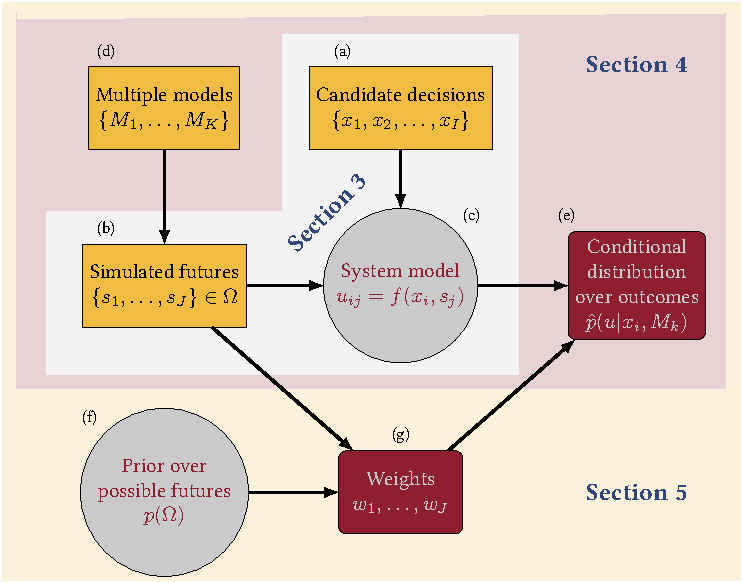
\includegraphics[width=\textwidth]{bayes-rdm.pdf}
    \caption{
        Outline of the proposed decision theoretic framework.
        Boxes are labeled in the order in which they are presented in the text.
        We begin in \cref{sec:multiple-simulation} using a lens of exploratory modeling, \ie boxes  (a), (b), and (c), to analyze the elevation problem.
        In \cref{sec:multiple-pdf} we discuss Boxes (d) and (e) to understand scenario-conditional probability distributions and the ``multiple \acrshort{pdf} problem''.
        Finally in \cref{sec:synthesizing} we add boxes (f) and (g) to synthesize across multiple \glspl{pdf}.
    }\label{fig:flowchart}
\end{figure}

\section{Exploratory analysis}\label{sec:multiple-simulation}

The literature on decision making under deep uncertainty \citep[see][]{marchau:2019} offers some insight as to how to identify decisions that perform well over many plausible \glspl{sow}.
We first consider exploratory modeling, which sheds light on the questions: ``how well does a given decision perform under different possible futures, and to which possible futures are different decisions vulnerable?''\james{Maybe this doesn't need to be a questino}


\Cref{fig:scenario-map} shows each possible future as a single point for each of several values of $\Delta h$.\james{Add after updating this figure}
On the $y$ axis is expected lifetime costs (see \cref{sec:sow-metrics}).
On the $x$ axis is mean sea level in 2100, which is an interpretable 1-dimensional projection of the \glspl{sow}.
Although our model for expected discounted total costs is deterministic, points with similar $x$-values may have different $y$-values because their sea levels before 2100 can differ (\ie, the 1-dimensional projection of the \glspl{sow} does not represent all variance between them).

\begin{figure}
    %\includegraphics[width=\textwidth]{scenario_maps.png}
    \caption{
        Scenario maps showing the dependence of average lifetime cost as a function of \gls{slr} in 2100 for several values of $\Delta h$.
        One dot represents one \gls{sow}.
        %TODO
    }\label{fig:scenario-map}
\end{figure}

The exploratory modeling approach shown in \cref{fig:scenario-map} shows that shows that the best outcome is when $\Delta h = 0$ and when \gls{slr} is negligible, but the worst outcome is also when $\Delta h = 0$ and when \gls{slr} is substantial.
As $\Delta h$ increases, the construction cost increases but the variability between different \glspl{sow} decreases, up to a point.
\emph{No decision dominates} any other, including $\Delta h = 0$, in the formal sense of being optimal over all \glspl{sow}.
\james{Revisit this paragraph once changes are made to \cref{fig:scenario-map}.}


\section{Scenario-conditional probabilistic analysis: the multiple PDF problem}\label{sec:multiple-pdf}

Whereas the analysis in \cref{sec:multiple-simulation} shed light on how decisions perform under different \glspl{sow}, the metrics calculated represent the performance of a given decision-\gls{sow} combination, and \emph{do not shed light on the performance of the decisions themselves}.

An alternative interpretation of the available \glspl{sow} is as \gls{iid} draws from each of eight \glspl{pdf} of sea level rise, as shown in \cref{fig:msl-boxplots}.
This has the approach of a probabilistic interpretation: \emph{conditional on a particular model} (\gls{rcp} scenario and ice sheet model structure), we can view corresponding \glspl{sow} as \gls{iid} draws from the distribution of outcomes.

A more formal notation is introduced in boxes (d) and (e) of \cref{fig:flowchart}.
Specifically, for each of $K$ models (box d), which here are our eight models for \gls{slr},\james{need to go through whole document and be consistent about MSL, SLS, SRL, RSLR, \etc} the samples of metrics are taken to be \gls{iid} samples from the distribution of outcomes (box e).
Since we define these models to estimate $p(\Omega)$, our models $M_1, \ldots, M_K$ return a probability of $1 / J_K$ for each of the $J_K$ simulations from the $K$th model, and $0$ for simulations from all other models.
We can then use this conditional distribution over outcomes to create metrics that depend only on the decision, such as averages or quantiles of outcomes.

\begin{figure}
    \centering
    %\includegraphics[width=2.5in]{tradeoffs_height_totalcost_byscenario.pdf}~
    %\includegraphics[width=2.5in]{tradeoffs_height_iqr_byscenario.pdf}
    \caption{
        Need a summary sentence.
        %TODO
        Trade-offs between (a) construction cost and expected lifetime costs or (b) construction cost and the uncertainty of future lifetime costs depend on the PDF selected.
    }
    \label{fig:tradeoffs}
\end{figure}

For example, \cref{fig:tradeoffs}(a) plots the expected lifetime cost\james{update figure} as a function of $\Delta h$\james{Add $\Delta h$ to the plot} for four of the eight models available.
Similarly, \cref{fig:tradeoffs} plots the 80\% confidence interval width (\ie, the 90th percentile minus the 10th percentile) of lifetime cost.
This figure shows that for small $\Delta h$, expected costs are low under optimistic models (\eg, \gls{rcp} 2.6 with slow ice sheet dynamics) and high under pessimistic models (\eg, \gls{rcp} 8.6 with fast ice sheet dynamics).
Consistent with \cref{fig:scenario-map}, the variability of lifetime costs increases as $\Delta h$ increases.
Once $\Delta h$ reaches \SIrange[]{3}{7}{ft}, depending on the model considered, construction costs start to dominate flood losses, and thus higher values of $\Delta h$ increase average lifetime costs.

Calculating either of the quantities shown in \cref{fig:tradeoffs} \emph{requires synthesizing across \glspl{sow}}.
However, these metrics are necessarily dependent on the model used (\ie, \gls{rcp} scenario and model of ice sheet dynamics).
This means that any assessment of decision performance (\eg, an optimal strategy, a Pareto frontier, or a cost-benefit analysis) is conditional upon an (explicit or implicit) model of future outcomes.
Where these models are implicit, they should be made more explicit to facilitate iterative model critique and improvement.

Second, this approach presents what we call ``the multiple \gls{pdf} problem'' because it leaves decision makers with many probability distributions to choose from
Cite \citet{sharma_rcp:2021} as another example.
Add a sentence or two explaining why this is a problem for decision makers\ldots\james{Need to bring in a bit of discussion from \citet{schneider_scenarios:2002} and from engineering docs (ASCE, FEMA, \ldots).}\klaus{Would appreciate your help putting together a succinct summary of the multiple \gls{pdf} problem}

\section{Synthesizing PDFs for decision relevance}\label{sec:synthesizing}

Motivated by the multiple \gls{pdf} problem, we develop in this section a framework for synthesizing information across \glspl{pdf} using subjective Bayesian modeling.\james{This also needs to go in the abstract}

Specifically, we frame the set of \glspl{sow} through a sampling lens and consider the possibility that the distribution from which they are sampled, $p_\textrm{empirical}(\Omega)$, does not reflect our belief about their true distribution, $p_\mathrm{true}(\Omega)$.
Often this is by design: exploratory modeling emphasizes the value of sampling low-probability futures as a way to learn about the system and develop insight \citep{bankes:1993}.\james{Tighten up this writing}
This is analagous to the deliberate over- or under-sampling of certain groups in survey design, and so following standard practice in survey design we develop a re-weighting approach to correct for the over- or under-sampling of different regions of the survey space.

We apply a grid-based discretization scheme to calculate these weights.
First, we project the \glspl{sow} $s_1, \ldots, s_J$ onto a one-dimensional space, which we denote $\psi_1, \ldots, \psi_J$.
As before, we take this space to be the mean sea level in 2100.
Without loss of generality, we assume the $\psi_j$ to be sorted from least to greatest so that $\psi_{j-1} \leq \psi_j$, ($j \neq 1$).
This allows us to simplify $p_\mathrm{true}(s_j) = p_\mathrm{true}(\psi_j)$.\klaus{This notation seems bad, suggestions?}
Defining $F_\mathrm{true}(s)$ to be the cumulative distribution corresponding to $p_\mathrm{true}$, \ie
$$F_\mathrm{true}(s) = \int_{-\infty}^{s'} p_\mathrm{true}(s) \dd{s},$$
we calculate weights using \cref{eq:weights} as illustrated in \cref{fig:weighting}.
\begin{equation}\label{eq:weights}
    w_j = \begin{cases}
        j = 1     & F_\mathrm{true}\qty(\frac{1}{2}\qty[\psi_1 + \psi_2])                                                                   \\
        1 < j < J & F_\mathrm{true}\qty(\frac{1}{2}\qty[\psi_{j} + \psi_{j+1}]) - F_\mathrm{true}\qty(\frac{1}{2}\qty[\psi_{j-1} + \psi_j]) \\
        j = J     & 1 - F_\mathrm{true}\qty(\frac{1}{2}\qty[\psi_{J-1} + \psi_J]).
    \end{cases}
\end{equation}
This grid-based weighting scheme can be used with higher-dimensional projections of the scenarios, as is done for example in the joint probability method used for hurricanes \citep[see, \eg,][]{johnson_clara:2013,toro_jpm-os:2010}.

The primary difficulty with \cref{eq:weights} is that the true probability distribution $p_\mathrm{true}(\phi)$ is deeply uncertain.
Because it is unknown, it must be approximated with a model.
And because it is deeply uncertain, multiple models\james{multiple priors?} for $p_(\Omega)$ should be used.
But whereas the $M_k$ defined in \cref{sec:multiple-pdf} represented the raw input data (four \gls{rcp} scenarios times two models of ice sheet dynamics), we define the $M_k$ here to be subjective models for mean sea level in 2100.\james{Are these models or priors?}

Need a few sentences here on prior uses of expert judgement and subjective belief.
The key point to get across is what a subjective belief means in the Bayesian context \citep{savage:1954,gelman_philosophy:2013,gelman_subjectiveobjective:2017}.
David Spiegelhalter had a nice comment on a podcast where he explained that in medicine, there isn't a ``true'' probability that, for example, you will get cancer; this is not some real quantity that can be measured \citep[hence the famous ``probability isn't real'' admonisment of][]{definetti_probability:1972}.
Similarly, the probability distribution of sea level rise in 2100 isn't something that can be measured.
However, probability provides a clear and self-consistent mathematical language for reasoning about uncertainty, which is why we're using it.
A key advantage is that \textbf{since we can't be right, we can at least be transparent} about the assumed values of sea level in 2100, rather than hiding behind implicit assumptions.
Thus we refer to the $M_k$ here as \emph{priors} to reflect that they consistently represent our current knowledge.

\begin{figure}
    \centering
    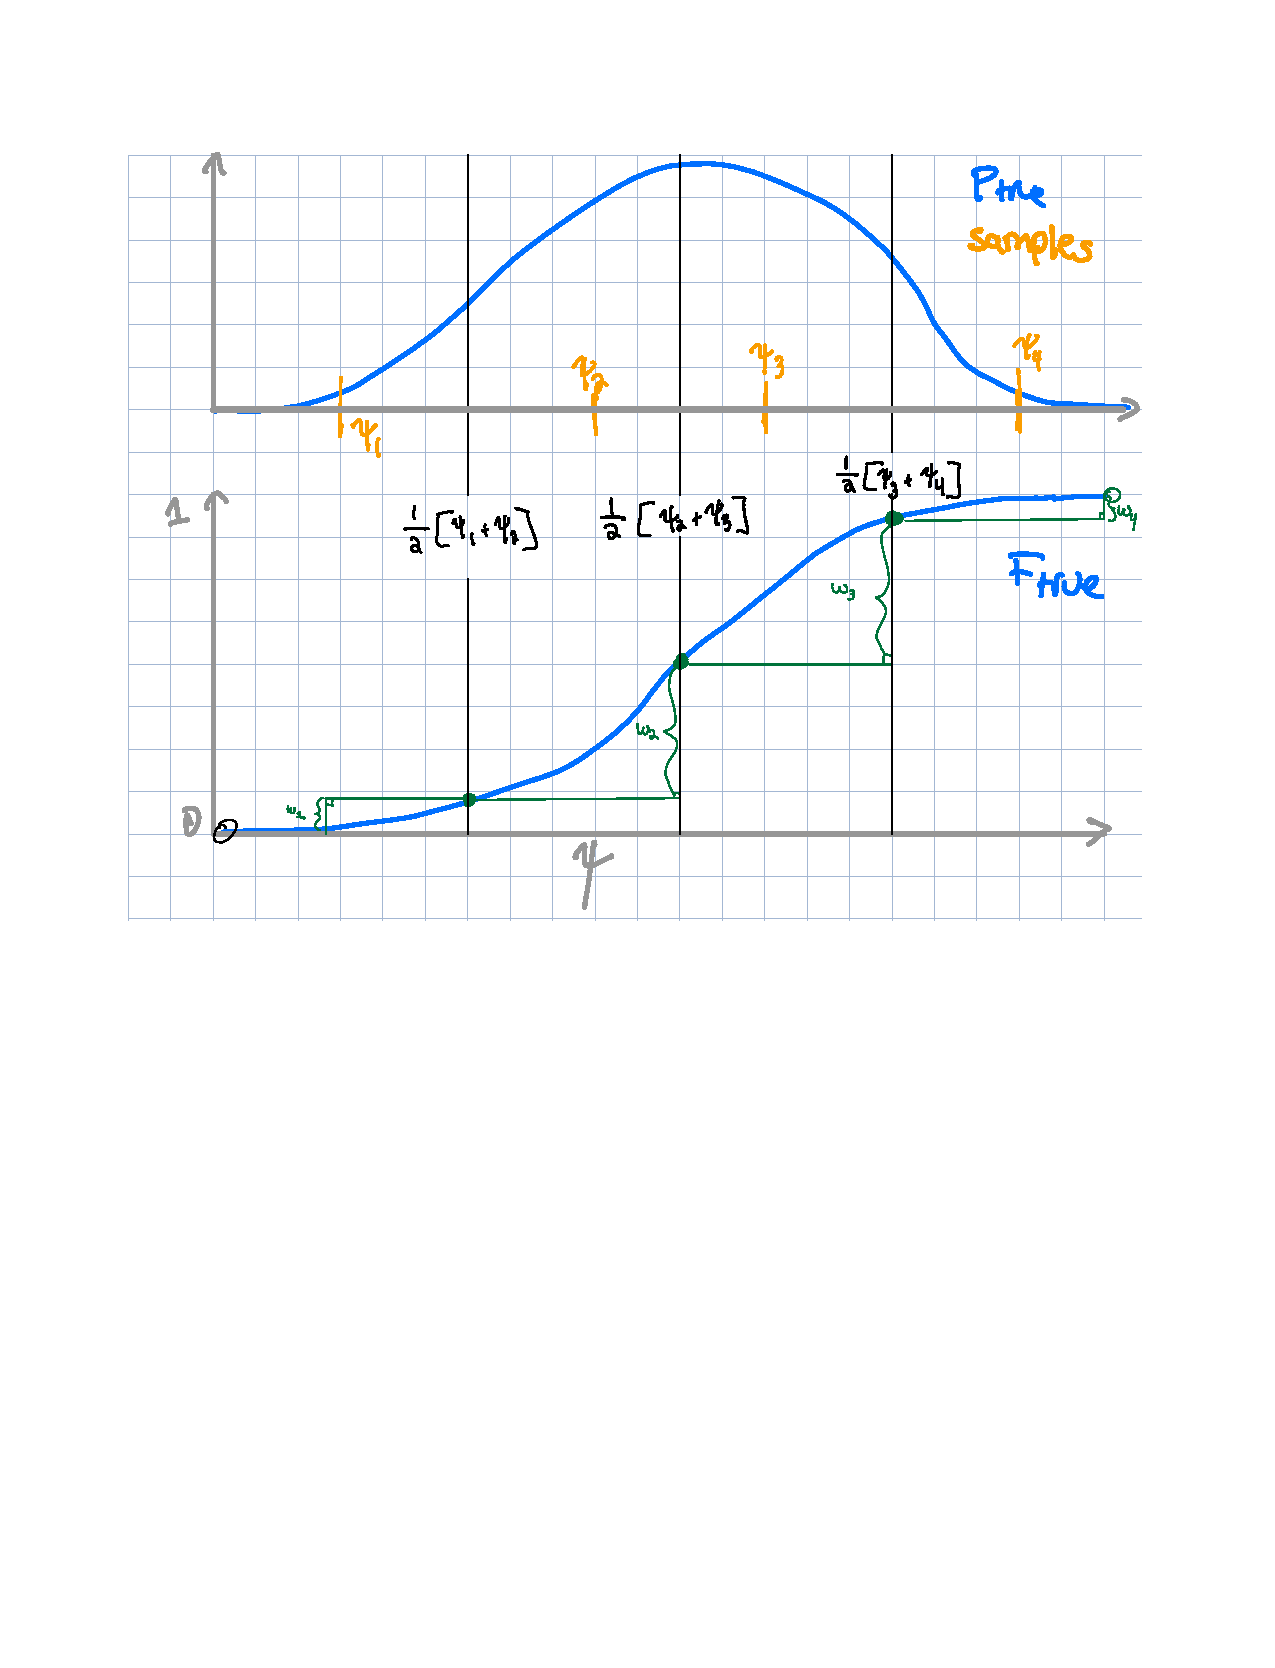
\includegraphics[width=4in]{../img/weighting.pdf}
    \caption{
        Schematic of re-weighting scheme defined in \cref{eq:weights} for $J=4$.
        Top panel shows $p_\mathrm{true}$ and bottom panel shows $F_\mathrm{true}$.
        Vertical black lines show $\frac{1}{2}\qty[\psi_j + \psi_{j+1}]$ for $j=1, \ldots, J-1$.
        Green text shows $w_1, \ldots, w_4$ and how they are calculated from $F_\mathrm{true}$.
        Need to update this figure using real data.
        %TODO
    }\label{fig:weighting}
\end{figure}

Need to explain how we came up with our two or three subjective priors.\klaus{Would love suggestions here!}
Another advantage of this method is that it is computationally cheap to re-weight the \glspl{sow}.
Thus, exploring performance under alternative priors is computationally cheap and easy to implement.
\Cref{fig:tradeoffs} shows the priors used in panel (a) and in panel (b) shows average lifetime cost as a function of the decision ($\Delta h$) after integrating over all possible \glspl{sow} (\ie, after synthesizing the ``multiple \glspl{pdf}.'')

\begin{figure}
    \centering
    %\includegraphics[width=3in]{lsl_priors.pdf}~
    %\includegraphics[width=3in]{tradeoffs_height_totalcost_byprior.pdf}
    \caption{
        The prior model averaging approach (\cref{fig:flowchart}), uses a probability distribution representing subjective belief to average insights across each PDF available.
        Alternative priors can provide robustness checks.
        Need to add panel labels, update data, \etc.
        %TODO
    }\label{fig:tradeoffs}
\end{figure}

This technique can also be used as a diagnostic tool.
In \cref{fig:model-average-weights}, we can see that the ``Pessimistic'' (``Optimistic'') prior heavily weights \gls{rcp} 8.5 (2.6), which is unlikely given current policies \citep{hausfather_scenarios:2020}.\james{Discuss a bit more}

\begin{figure}
    \centering
    %\includegraphics[width=6in]{inference_weights.pdf}
    \caption{
        The average weight assigned to \glspl{sow} from each model (\gls{rcp} scenario and ice sheet parameterization) for both priors considered.
        If the sampling distribution (green line) is used, then the weight assigned to each \gls{sow} is the same, regardless of whether it is over- or under-sampled.
    }\label{fig:model-average-weights}
\end{figure}


\section{Conclusions}\label{sec:conclusions}

To summarize:
\begin{itemize}
    \item Natural extensions to Bayesian updating
    \item Belief $p(s)$ can't be ``right''  \citep{gelman_workflow:2020,gelman_philosophy:2013} or ``neutral'' \citep{quinn_exploratory:2020}
\end{itemize}

This didactic example illustrates a need for better synthesis and communication of deep uncertainties for decision making.

Future research needs:
\begin{itemize}
    \item More complex models to capture more relevant metrics
    \item Better models of nonstationary hazards
    \item Interacting, sequential decisions
\end{itemize}

\section{Bonus (need to sort through)}

This section is a work in progress -- it includes some text that used to be in the paper as well as some bullet points that may be useful for the discussion section.\klaus{Can you highlight any picese here that you find especially salient?}

Including additional models \citep[\eg,][]{kopp_evolving:2017,deconto_antarctica:2016,ruckert_coastal:2019} \emph{would compound this challenge}.\james{Lee et al: Lee, Haran, Pollard, Keller}

Most fundamentally, we are thinking about robustness a bit differently than usual.
The typical way that the DMDU literature thinks about it is robustness to a \gls{sow}.\james{This is a simplification}
We are thinking about robustness to different modeling structures and assumptions.
This has links to the ``rival framings'' literature.
Given a subjective prior $p(s)$, I can compute expectations of the decision metrics $m$; if there are a lot of decisions, I can start to sketch out the trade-off curves as shown in figures XXXX (in \cref{sec:results}).

Since we have priors, there are clear links to how we would update our belief (and thus decision) once more information arrives.

\begin{enumerate}
    \item Links to DMDU literature
          \begin{enumerate}
              \item We should also cite \citet{quinn_exploratory:2020}, which makes the point that it matters how you sample \glspl{sow}.
              \item Exploratory modeling can help to demonstrate the existence of particular outcomes, generate hypotheses, build qualitative insight, and identify scenarios worthy of further study \citep[see][]{bankes:1993}.
              \item You can do scenario discovery
              \item We are in effect calculating robustness metrics \citep{mcphail_robustness:2019,herman:2015}
          \end{enumerate}
    \item Philosophy of Bayesian stats / decision making
          \begin{enumerate}
              \item The observation that many of these mechanisms cannot be represented by a single objective \gls{pdf} has motivated many criticisms of the application of \gls{bdt} to planning problems.\james{Cite some (from thesis)}
                    Yet \gls{bdt} was conceived as a calculus for reasoning rather than for identifying objective truth; \citeauthor{definetti_probability:1972} often said that ``probability does not exist'' \citeyear{definetti_probability:1972}.
                    \citet{savage:1954} and \citet{ramsey_probability:2016}, among others, also viewed probability as ``subjective,'' representing the state of belief of the decision-maker.
                    The famous phrase ``all models are wrong, but some are useful'' \citep[generally attributed to][]{box:1976} also suggests that probability distributions and predictions ought to be viewed subjectively.
                    More recent discussions of Bayesian philosophy \citep{jaynes_probability:2003,McElreath:2016vu,Gelman:2014tc,bernardo_bayesian:1994} also emphasize a philosophical view of probability as a language with which to reason about the unknown rather than a statement of objective truth \citep[see][for a thorough discussion of Bayesian philosophy]{gelman_philosophy:2013}.\klaus{Am I reading right that you say ``maybve have this in intro to motivate the analysis?''}
                    Although the true data generating process is not known and inference should not be represented as objective truth, probability gives a transparent and consistent language for reasoning about uncertainty.\james{This should go to intro}
                    Since modeling assumptions cannot overcome epistemic uncertainty, even with better models and more data, we draw from the literature on statistical model selection in the $\mathcal{M}$-open setting, which provides a theoretical background for choosing between models when the true data generating process is not among the models considered \citep[see][]{Piironen:2017eh}.\james{Explain this to the audience}
                    Often, combining inferences from multiple models is more effective than seeking a single ``best'' model \citep{Yao:2018bu}.
                    More fundamentally, this literature emphasizes the importance of iteratively building models, simulating the consequences of those models, and critiquing them \citep{gelman_workflow:2020}.
                    Since, by definition, models are not ``true,'' this iterative workflow aims to identify models that are useful and promote a dialog amongst stakeholders \citep{gelman_philosophy:2013}\footnote{this paragraph is copied from my dissertation, needs to be re-worked!}
          \end{enumerate}
    \item There are interesting links to Bayesian model averaging
          \begin{enumerate}
              \item Lots of examples to cite if we want
              \item I'm partial to something like stacking \citep{Yao:2018bu}
              \item The main difference is we are using only the prior to average the models!
          \end{enumerate}
    \item Limitations of the case study
          \begin{enumerate}
              \item Objectives: real people might care about uncertainty (risk aversion), probability of experiencing flooding at all (disruptions are hard to quantify), usable space created under the house, and more
              \item More uncertainty (damage functions, cost of construction, lifespan, discount rate, \etc)
              \item Better data on cost of elevation and depth-damage
              \item Robustness: ptimize separately for different kinds of house structures and locations
              \item Timing
          \end{enumerate}
    \item Limitations of the method
          \begin{enumerate}
              \item Our prior $p(s)$ is limited -- we are just using \gls{lsl} in 2100 but we could be looking at more parameters of it including rate of change, \etc
              \item We neglect true ignorance \citep{knight_risk:1921}.\james{Perhaps ``unknown unknowns''}
              \item The real world is in a state of ``unknown unknowns'' \citep[level 5 as defined in][fig.~1]{walker_deep:2013} so trying to represent \emph{all} uncertainty is futile; we must make subjective modeling choices and assumptions about what is most important
          \end{enumerate}
    \item The benefits of this approach:
          \begin{enumerate}
              \item A goal is to make imperfect and subjective modeling choices as transparent as possible. Since we can't be right, we should make it as easy as possible for others to understand and critique our assumptions\james{Focus on this!}
              \item Because of how we weight realizations of the future, you can apply a different weighting function and immediately assess performance. Thus qualitative and quantitative sensitivity analyses are simple.
              \item Of course the choice of $p(\mathcal{Z})$ is subjective, but so is every other aspect of how we frame the problem. Modeling is intrinsically subjective. The idea of embracing subjective choices -- and making them explicit and open to critique -- draws heavily from philosophies of iterative workflow in statistics \citep{box:1976,gelman_workflow:2020,gelman_philosophy:2013}.
              \item This approach can be used in a multiobjective context and is an alternative way to measure robustness in \gls{rdm} and MORDM
          \end{enumerate}
    \item This approach can be used in many other contexts
          \begin{enumerate}
              \item Direct
                    \begin{enumerate}
                        \item Stormwater management \citep{sharma_rcp:2021,lopez-cantu:2018}
                        \item Levee heightening \citep{garner_slrise:2018,oddo_coastal:2017,vandantzig_dike:1956}
                    \end{enumerate}
              \item Indirect
                    \begin{enumerate}
                        \item Lots of economic models like social cost of carbon or effect of policy on metrics of interest make assumptions about deep uncertainties!\james{Let's emphasize this -- really important to policy analysis under deep uncertainty}
                        \item Model structure uncertainties
                    \end{enumerate}
          \end{enumerate}
\end{enumerate}.

Federal guidance for this decision relies on standards (the $T$-year flood) rather than risk-based design.
Be sure to note that this has parallels to lots of other engineering design guidance.
Then note the work of \citet{zarekarizi_suboptimal:2020} and \citet{xian_elevation:2017} who show that a risk-based approach may improve significantly on a standards-based approach.\james{Need to addd some citations of ``risk-based design''}

Additionally, the floodplain maps used for decision support are silent on projected future changes and neglect the deep and dynamic uncertainties surrounding the projected hazards\ldots
Both risk-based design and standards-based approaches are complicated by nonstationarity.
On the one hand, nonstationarity of flood hazard is already evident in many places, especially in coastal areas where \gls{slr} is clear.
On the other, efforts to find objective methods for quantifying nonstationarity, \eg of precipitation \citep{atlas14_texas:2018} or flood frequency \citep{bulletin17c:2019}, have struggled to find a satisfactory approach because factors like future emissions and localized climate response create deep uncertainties that resist objective quantification \citep[see][]{keller_management:2021}.\james{This goes earlier -- see Klaus's added text}

This suggests that either nonstationarity should be ignored, or subjective approaches for designing for nonstationarity should be adapted.
Given that physical theories consistent with the observational record and models robustly project changes to climate hazard under warning,

Many methods for decision making under deep uncertainty first evaluate candidate decisions over many plausible states of the world, then aggregate performance over these possible futures.
Through a didactic case study of determining how high to elevate a single home in Norfolk, VA, we demonstrate that the common practice of weighting all scenarios equally in this aggregation creates a tension between (a) fully exploring the parameter space, including unlikely regions, and (b) accurately representing available scientific knowledge.
We introduce an approach to bridge this divide through a computationally efficient method that weights each state of the world based on a probability distribution over possible futures.
Since the distribution of deeply uncertain variables is necessarily subjective, we turn to frameworks for model critique from applied Bayesian statistics to compare and contrast different modeling assumptions.
This approach can help to improve decision-making by facilitating iterative and collaborative model improvement.

While classical utility- or regret-based frameworks offer a structure for weighing these risks, they are not designed to handle uncertainties that are \emph{deep} in the sense that stakeholders may not agree upon their probabilities \citep{lempert_complex:2002} or \emph{irreducible} in the sense that there is not an objective truth that better models and data can identify \citep{DossGollin:2019}.\footnote{Unless we believe everything is pre-determined, in which case why bother with climate adaptation\ldots}
Examples of such uncertainties include how much greenhouse gasses humans will emit in the future or whether the U.S. federal government will continue to subsidize flood insurance for homeowners.\james{Add some references}
In response, a wide range of fields have developed scenario-based methods\ldots.\klaus{Which arguments in \citet{savage:1954} did you think should be cited here?}
This leads to the ``Multiple PDF Problem'' \citep{sharma_rcp:2021}\ldots.
A key question, then, facing the designers, builders, regulators, owners, and users of built facilities is \emph{to which scenario should infrastructure be designed?}

One example is building codes and guidelines\ldots.
Prior studies have found that floodproofing and building-scale vulnerability reduction measures, including house elevation, can effectively reduce local flood damages in many contexts \citep{demoel_reducing:2014,deruig_building:2020,kreibich_building:2005,slotter_floodproofing:2020,Rozer:2016dn,mobley_mitigation:2020,aerts_cost:2018}.
Official guidance for homeowners, notably from \gls{fema}, recommends elevating to the \gls{bfe} (typically the \SI{100}{year} flood) plus a freeboard \citep{fema_retrofitting:2014,asce_24-14:2015,fema_retrofitting:2014} but recent suggests scope for improvement.
For example, \citet{xian_elevation:2017} used a cost-benefit analysis to demonstrate that tailoring recommendations to the inital elevation of a structure can reduce expected costs.
\citet{zarekarizi_suboptimal:2020} show that neglecting uncertainty in discount rate, house lifespan, flood risk, and depth-damage curves can lead to maladaptation.
Yet these studies are silent on the question of how nonstationary flood hazard should factor into this decision.

Nonstationarity is particularly relevant in coastal communities where \gls{slr} is expected to drive future flood risk.
As a didactic case study, we consider the problem of how high a homeowner should elevate their structure to mitigate future flood losses, illustrated in \cref{fig:house-sketch},\james{Need to revisit this picture} given stochastic flood peaks and deeply uncertain \gls{slr}.
\Gls{slr} is driven mainly by physical processes like (\ldots, West Antarctic Ice Sheet, \ldots\klaus{You wrote something here that I can't read -- I see something that looks like ICM. I assume Tony and Kelsey papers are relevant as well?}) \citep{kopp_probabilistic:2014,kopp_evolving:2017}.
Two key uncertainties identified by previous studies are
\begin{enumerate*}[label=(\roman*)]
    \item which emissions pathway (\eg, \gls{rcp} scenario) will we experience and
    \item how will polar ice sheets respond to warming \citep{wong_brick0.2:2017,ruckert_coastal:2019,wong_nola:2017,deconto_antarctica:2016}.
\end{enumerate*}
Simulations of \gls{slr} are available to decision makers grouped by \gls{rcp} scenario and model structure.
For a given combination of \gls{rcp} scenario and model, results are typically presented and interpreted as probabilistic, but this is not the same as giving decision-makers a single \gls{pdf}.
This is the ``Multiple \gls{pdf} Problem'' described in, \eg, \citet{sharma_rcp:2021}.
Thus, \emph{which scenario/\gls{pdf} should we design for?}

Lacking a crystal ball capable of telling us precisely which \gls{pdf} we need to design for, we have to consider several as plausible.
Any decision will perform differently in different scenarios.
There is no objective answer to this question.
Since we can't be ojectively correct, we might as well be transparent and make our assumptions explicit (and subject to critique) rather than implicit.

Households elevate their homes to manage flood risks, but regulations and guidance are silent on key questions \citep{zarekarizi_suboptimal:2020,xian_elevation:2017}.
\begin{description}
    \item[Q1] How to adapt guidance to building characteristics or household preferences?
    \item[Q2] How does nonstationary hazard change guidance?
    \item[Q3] Which model of nonstationary hazard to use?
\end{description}
These challenges also affect other adaptation plans and engineering designs (\cref{fig:stormwater-bridge}).

\section*{End Matter}

\begin{enumerate}
    \item Supplementary figures and analysis online
    \item Link to live repository on GitHub
    \item Link to code DOI on Zenodo
\end{enumerate}

\subsection*{Acknowledgements}

\begin{enumerate}
    \item MARISA\james{details}
    \item PSIRC\james{details}
    \item Rice University (for startup)
    \item Dartmouth College (for startup)
    \item Tor Erlend Fjelde for helpful advice on implementing the \gls{gev} prior using \texttt{Turing.jl}.
    \item For many journals, a code and data statement will go here.\james{Keep an eye on this}
\end{enumerate}

\subsection*{Author Contributions}

See journal requirements and format\james{Keep an eye on this}

\printbibliography

\appendix
\newcommand{\hbAppendixPrefix}{S}
\renewcommand{\thefigure}{\hbAppendixPrefix\arabic{figure}}
\setcounter{figure}{0}
\renewcommand{\thetable}{\hbAppendixPrefix\arabic{table}}
\setcounter{table}{0}
\renewcommand{\theequation}{\hbAppendixPrefix\arabic{equation}}
\setcounter{equation}{0}

\newpage
\section{Supplemental figures}
\begin{figure}
    \centering
    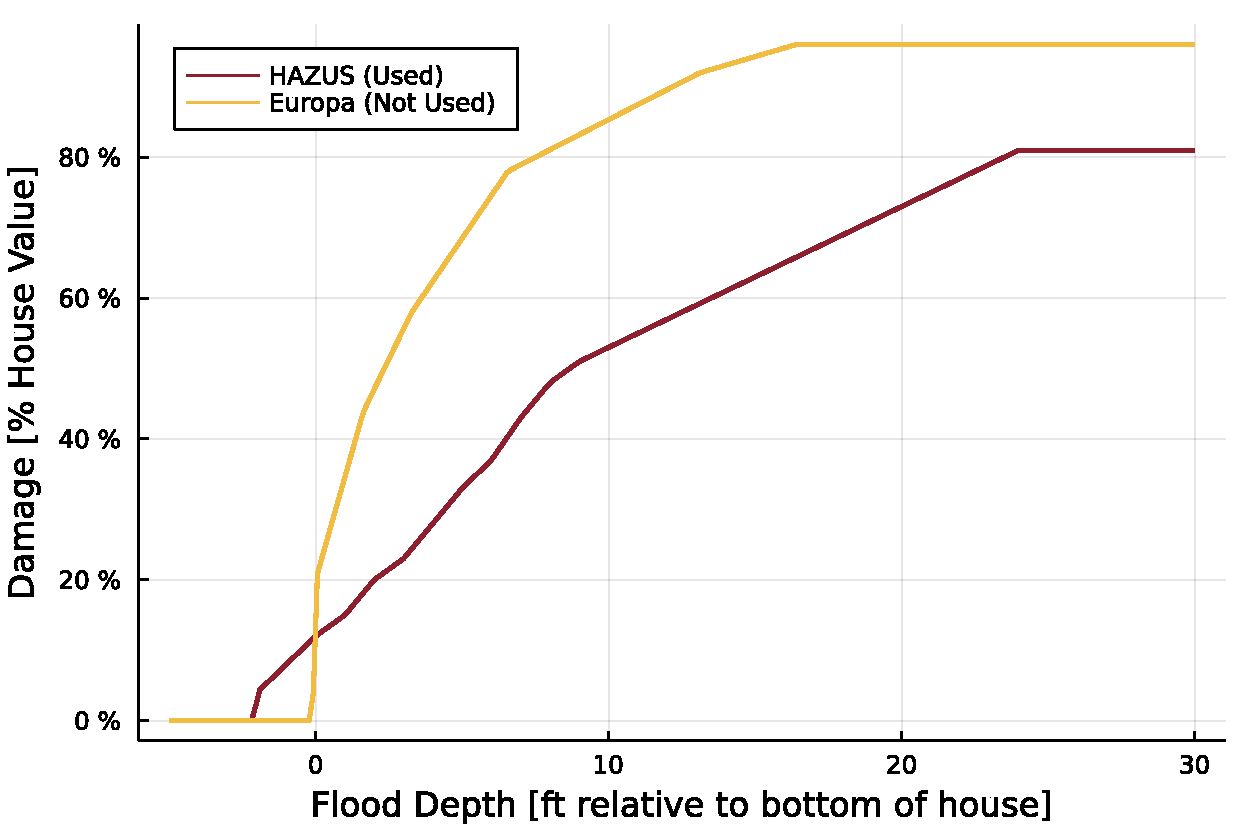
\includegraphics[width=4in]{cost-depth-damage}
    \caption{
        Depth-damage relationship.
        Following \citet{zarekarizi_suboptimal:2020}, we use the Hazard U.S. (HAZUS) depth-damage curves provided by FEMA.
        Since results are sensitive to choice of depth-damage equation, we illustrate (for comparison only) the ``Europa'' depth-damage relationship developed by the Joint Research Center (JRC) of the European Commission's science and knowledge service \citep{huizinga_depthdamage:2016}.
    }\label{fig:cost-depth-damage}
\end{figure}

\begin{figure}
    \centering
    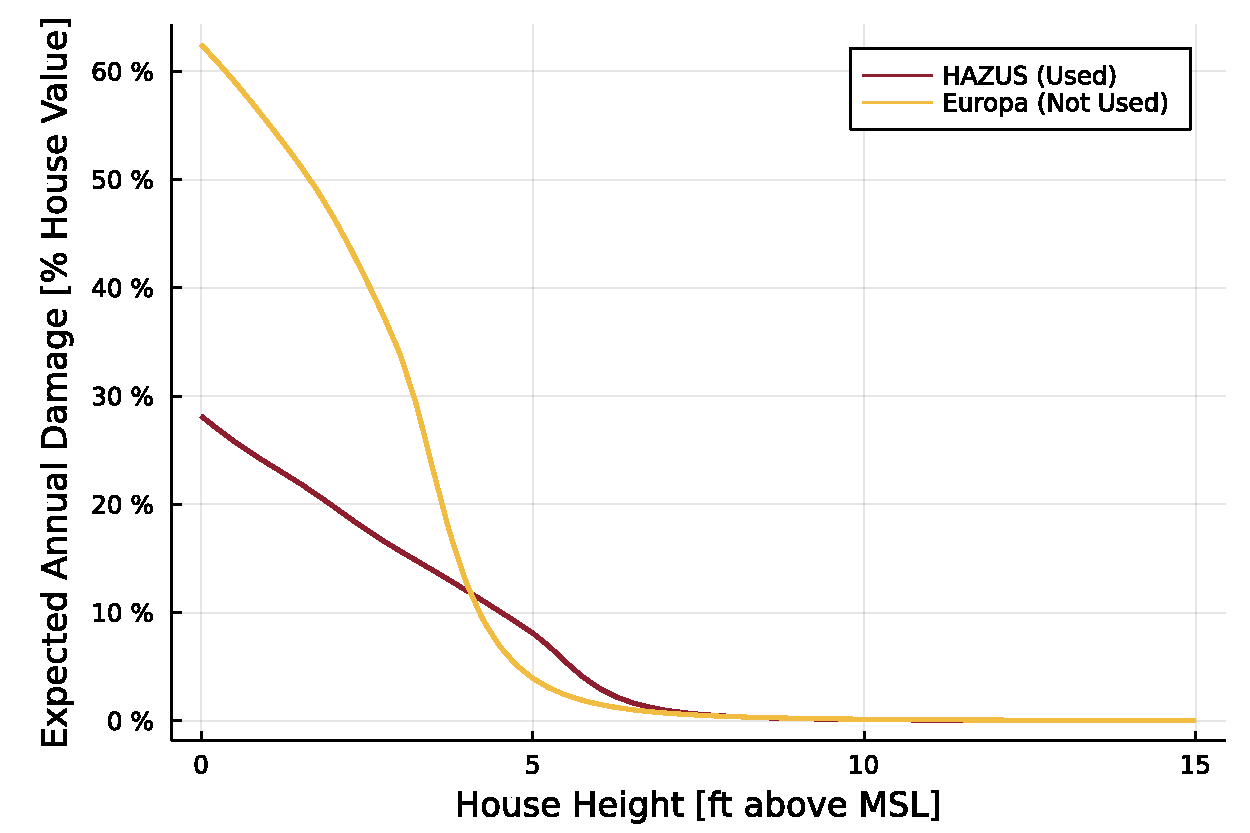
\includegraphics[width=4in]{cost-expected-damage-emulator}
    \caption{
        As discussed in XXX, we model expected annual damages as a function of the house's elevation relative to \gls{lsl}. % TODO: ref equation
    }\label{fig:cost-expected-damage-emulator}
\end{figure}

\begin{figure}
    \centering
    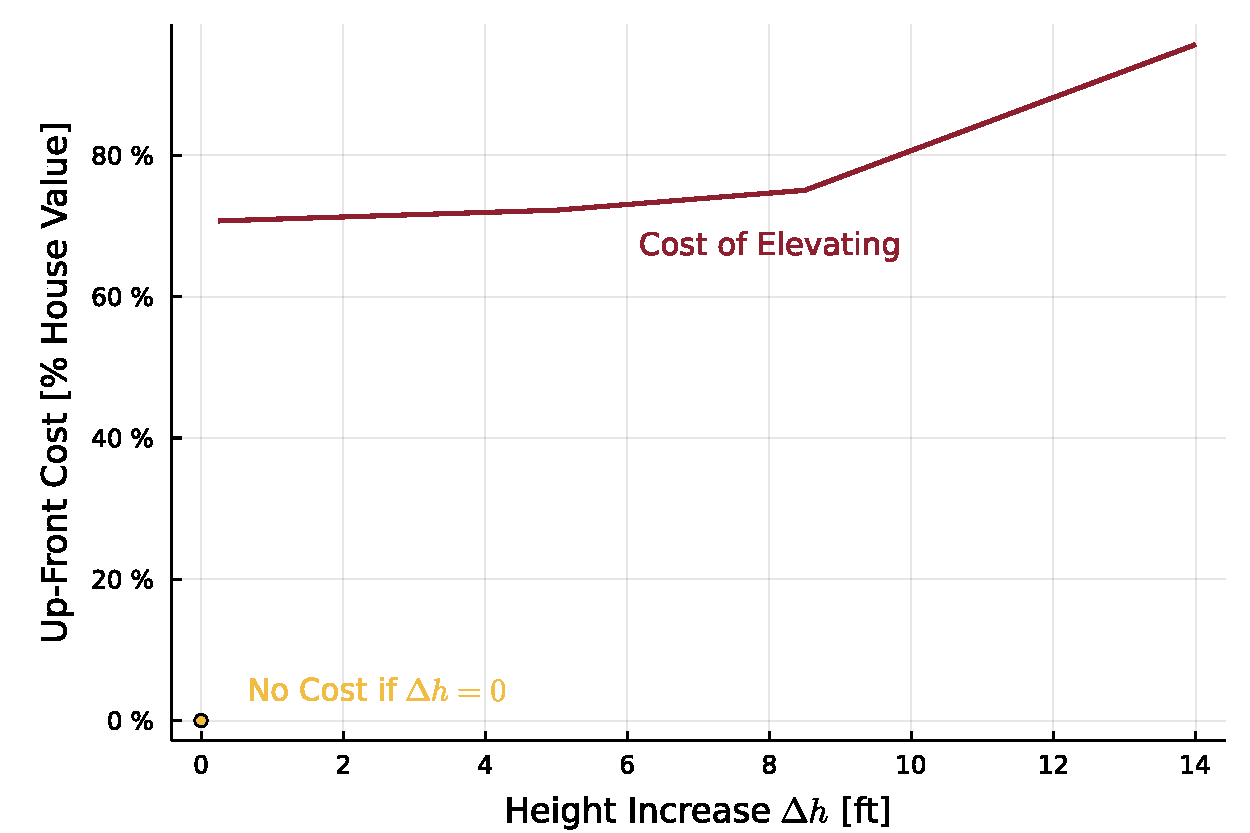
\includegraphics[width=4in]{cost-up-front}
    \caption{
        Following \citet{zarekarizi_suboptimal:2020}, we model the cost of elevating a single-family house by interpolating estimates from the Coastal Louisiana Risk Assessment Model \citep{johnson_clara:2013}.
        According to this model, the unit cost of elevating a house by 3-7, 7-10, and 10-14 feet is \usd{82.50}, \usd{86.25}, and \usd{103.75} per square foot, respectively, with a \usd{20745} initial fee.
        Values are sensitive to house floor area and structural value; see \cref{tab:uncertainties}.
    }\label{fig:cost-up-front}
\end{figure}

\begin{figure}
    \centering
    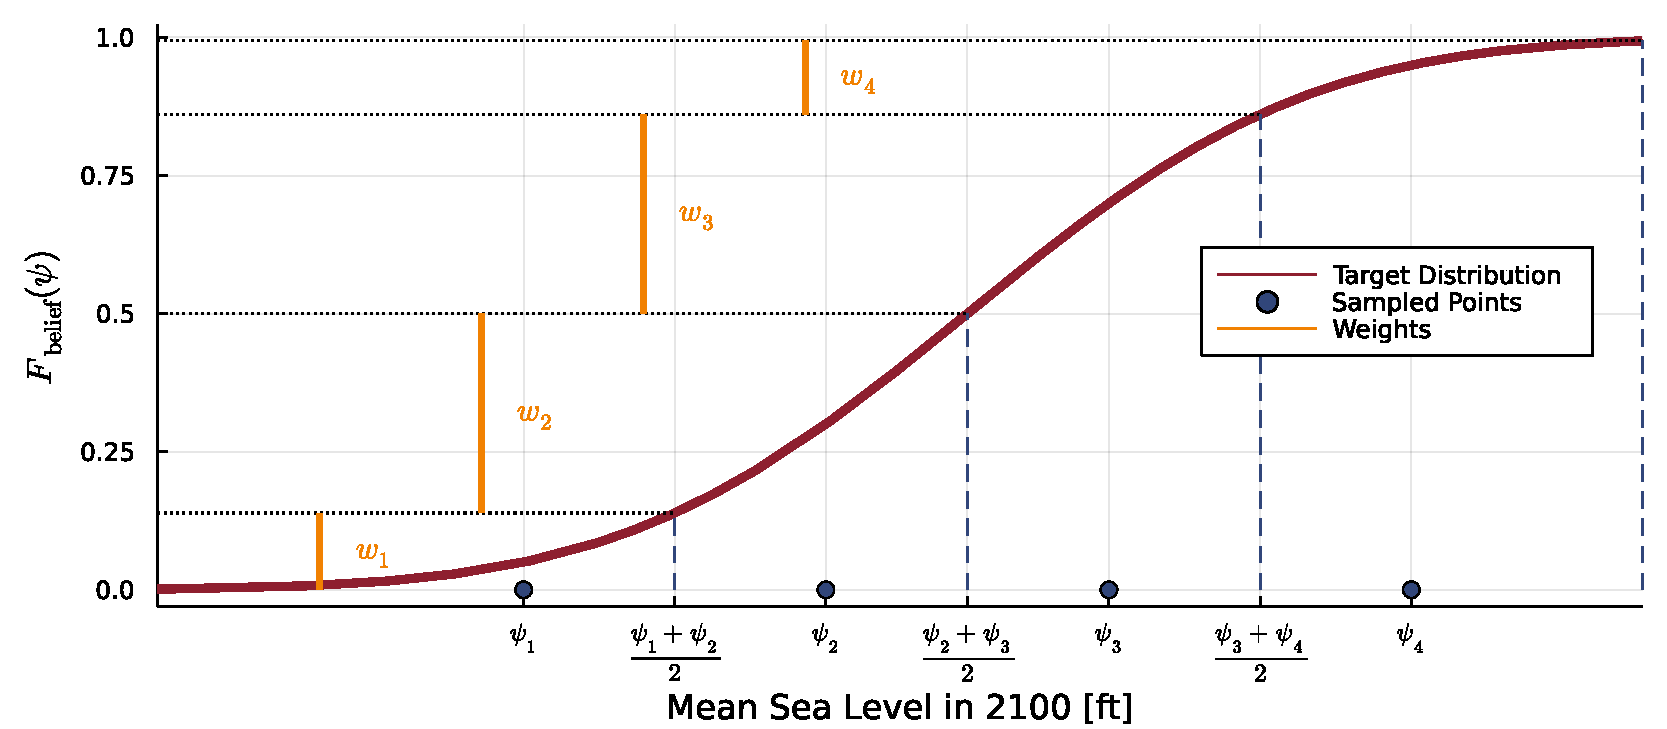
\includegraphics[width=4in]{grid-sketch}
    \caption{
        Schematic of equation XXX used to calculate weights for each sample. % TODO: reference equation
        This method is illustrated for a hypothetical target distribution (orange line) and four samples $\psi_1, \psi_2, \psi_3, \psi_4$ (blue dots).
        As discussed in section XXX, the weights (vertical blue lines) are calculated based on the \gls{cdf} of the target distribution  (horizontal dotted lines) at the halfway points $\frac{1}{2}\qty[\psi_i+\psi_{i+1}]$ (vertical dashed lines). % TODO: reference section
    }\label{fig:grid-sketch}
\end{figure}

\begin{figure}
    \centering
    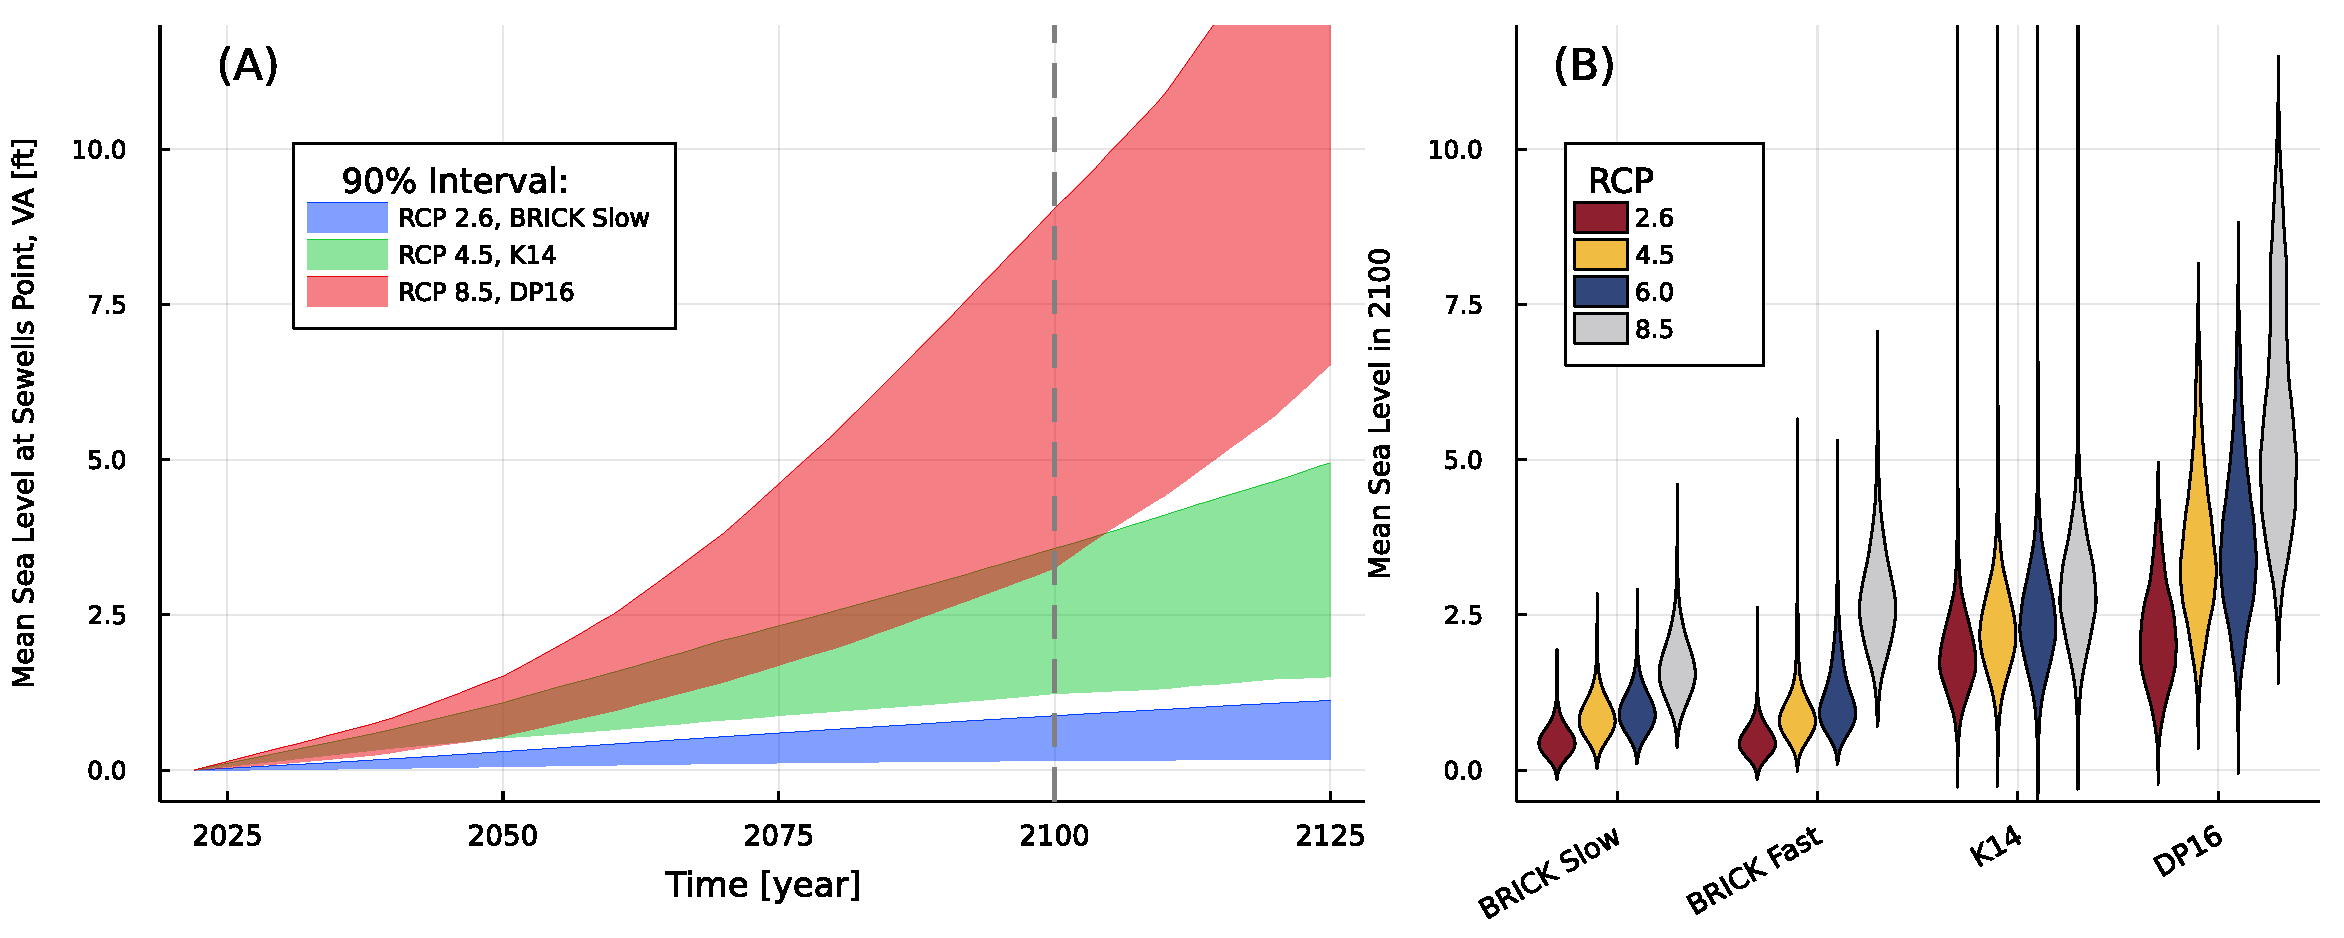
\includegraphics[width=\textwidth]{lsl-evolution}
    \caption{
        Projections of future mean sea level depend strongly on the model (\gls{rcp} scenario and physical representation) used.
        (A): 90\% intervals for mean sea level at Sewells Point, VA as a function of time for three probabilistic models.
        (B): probability distribution of mean sea level at Sewells Point, VA in the year 2100 for all probabilistic models considered.
    }\label{fig:lsl-evolution}
\end{figure}

\begin{figure}
    \centering
    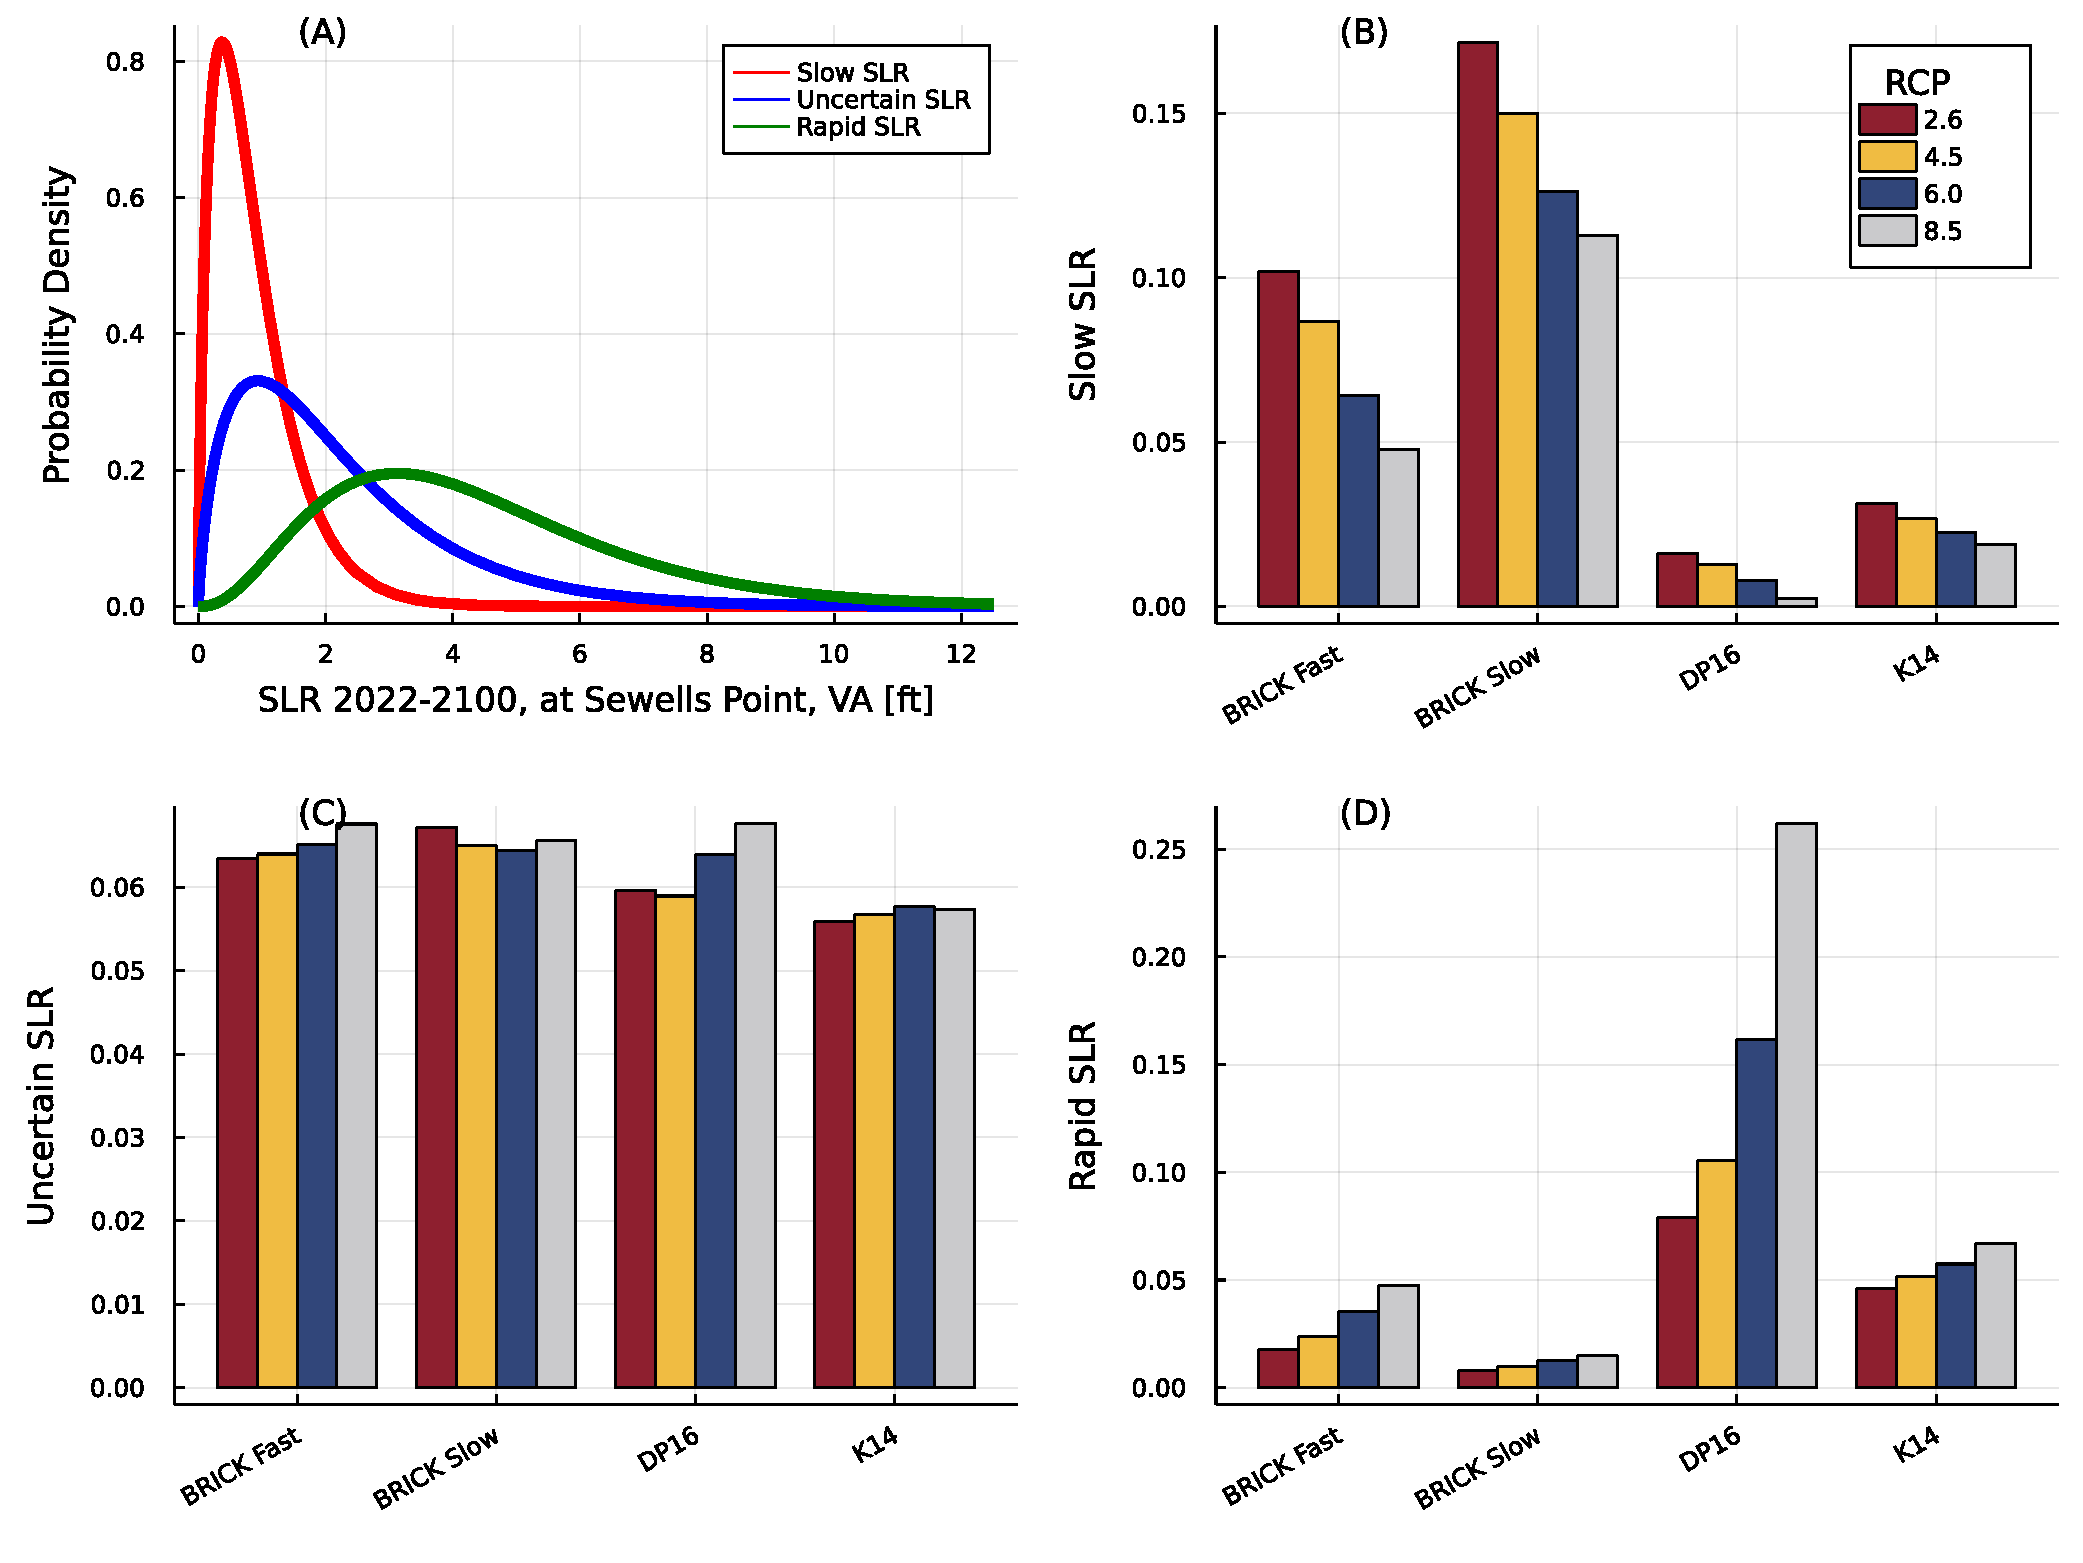
\includegraphics[width=\textwidth]{lsl-priors-weights}
    \caption{
        Subjective priors for local sea level.
        We develop three distributions (``subjective priors'') representing plausible probabilistic beliefs about \gls{lsl} at Sewells Point, VA in 2100, relative to the present.
        The \glspl{pdf} of these subjective priors are shown in panel (A).
        In panels (B)-(D), we show the relationship between these subjective priors and the 16 probabilistic models (four \gls{rcp} scenarios and four physical representations) available.
        Specifically, (B)-(D) show the average weight given to each model by each of the three subjective priors.
        The ``Slow SLR'' prior places large weight on BRICK model \citep{wong_brick0.2:2017}, particularly the scenarios with no fast ice sheet dynamics and on low-emissions scenarios.
        The ``Fast SLR'' prior places most of its weight on the \citet{deconto_antarctica:2016} model, and in particular on high-emissions scenarios.
        The ``Intermediate SLR'' scenario places approximately equal weight on all models.
    }\label{fig:lsl-priors-weights}
\end{figure}

\begin{figure}
    \centering
    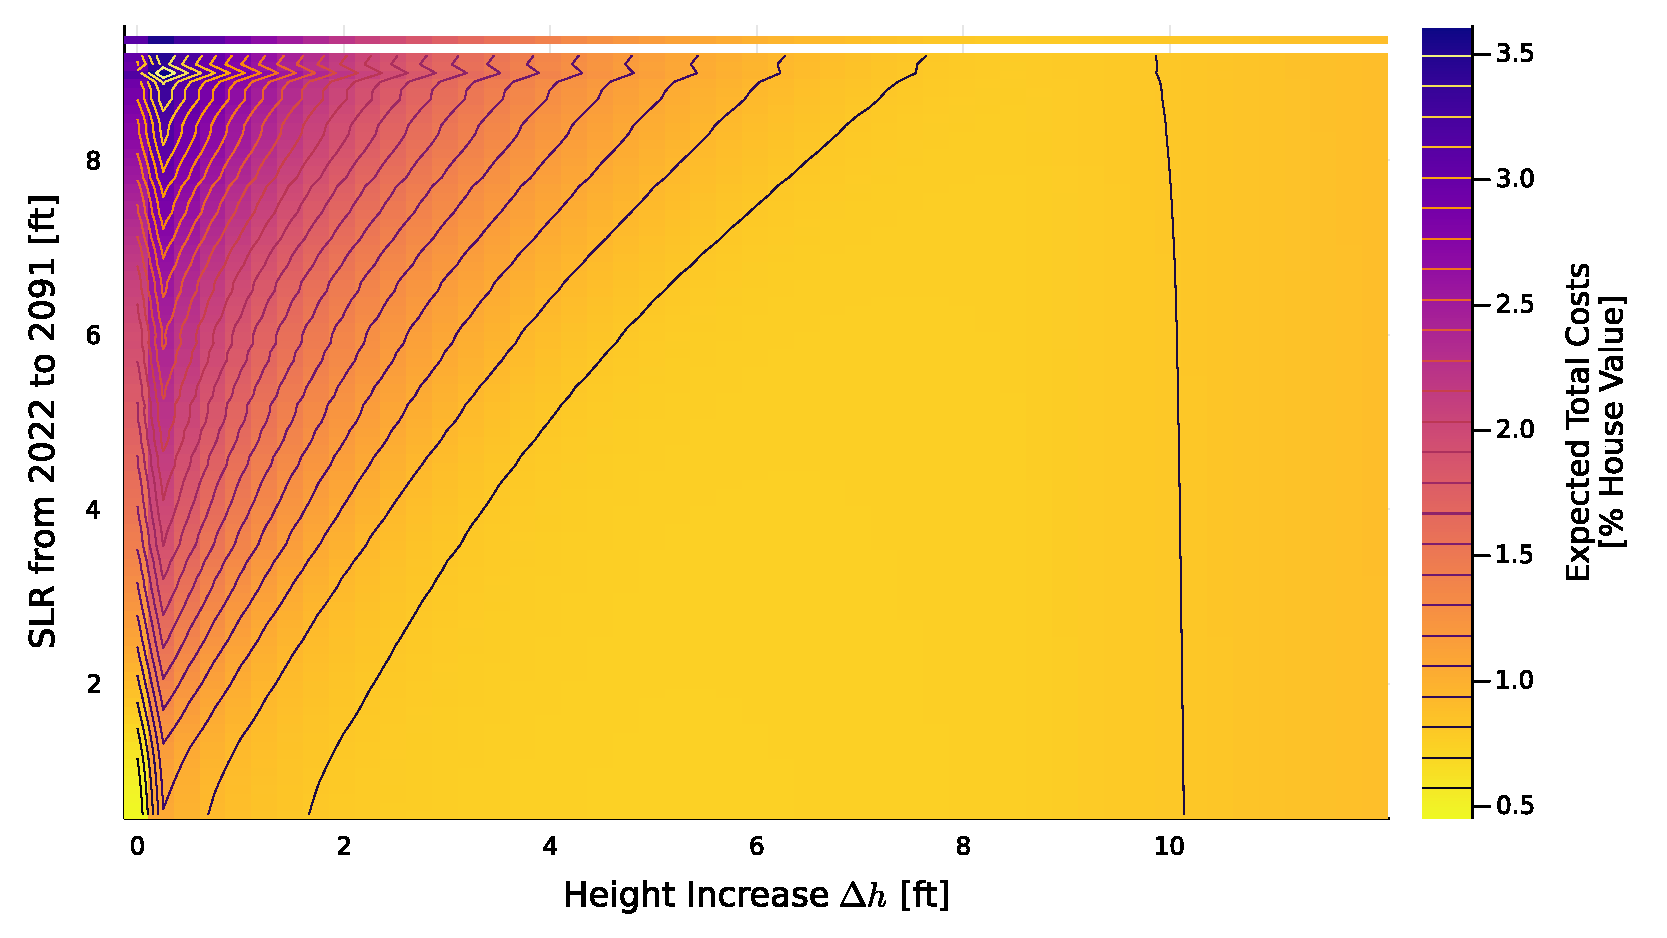
\includegraphics[width=\textwidth]{scenario-map-height-slr}
    \caption{
        Expected total lifetime cost (damages plus up-front cost; eq.XXX) as a function of height increase $\Delta h$ and sea level rise over the house lifetime. % TODO: reference equation
        The best outcomes (yellow) arise when the house is not elevated and sea level rise is minimal (bottom left corner).
        The worst outcomes (blue) arise when the house is elevated only slightly and sea level rise is rapid.
        In general, a height increase of $<\SI{3}{ft}$ can be considered unrealistic \citep{zarekarizi_suboptimal:2020}.
        Values are sensitive to model constants; see \cref{tab:uncertainties}.
    }\label{fig:scenario-map-height-slr}
\end{figure}

\begin{figure}
    \centering
    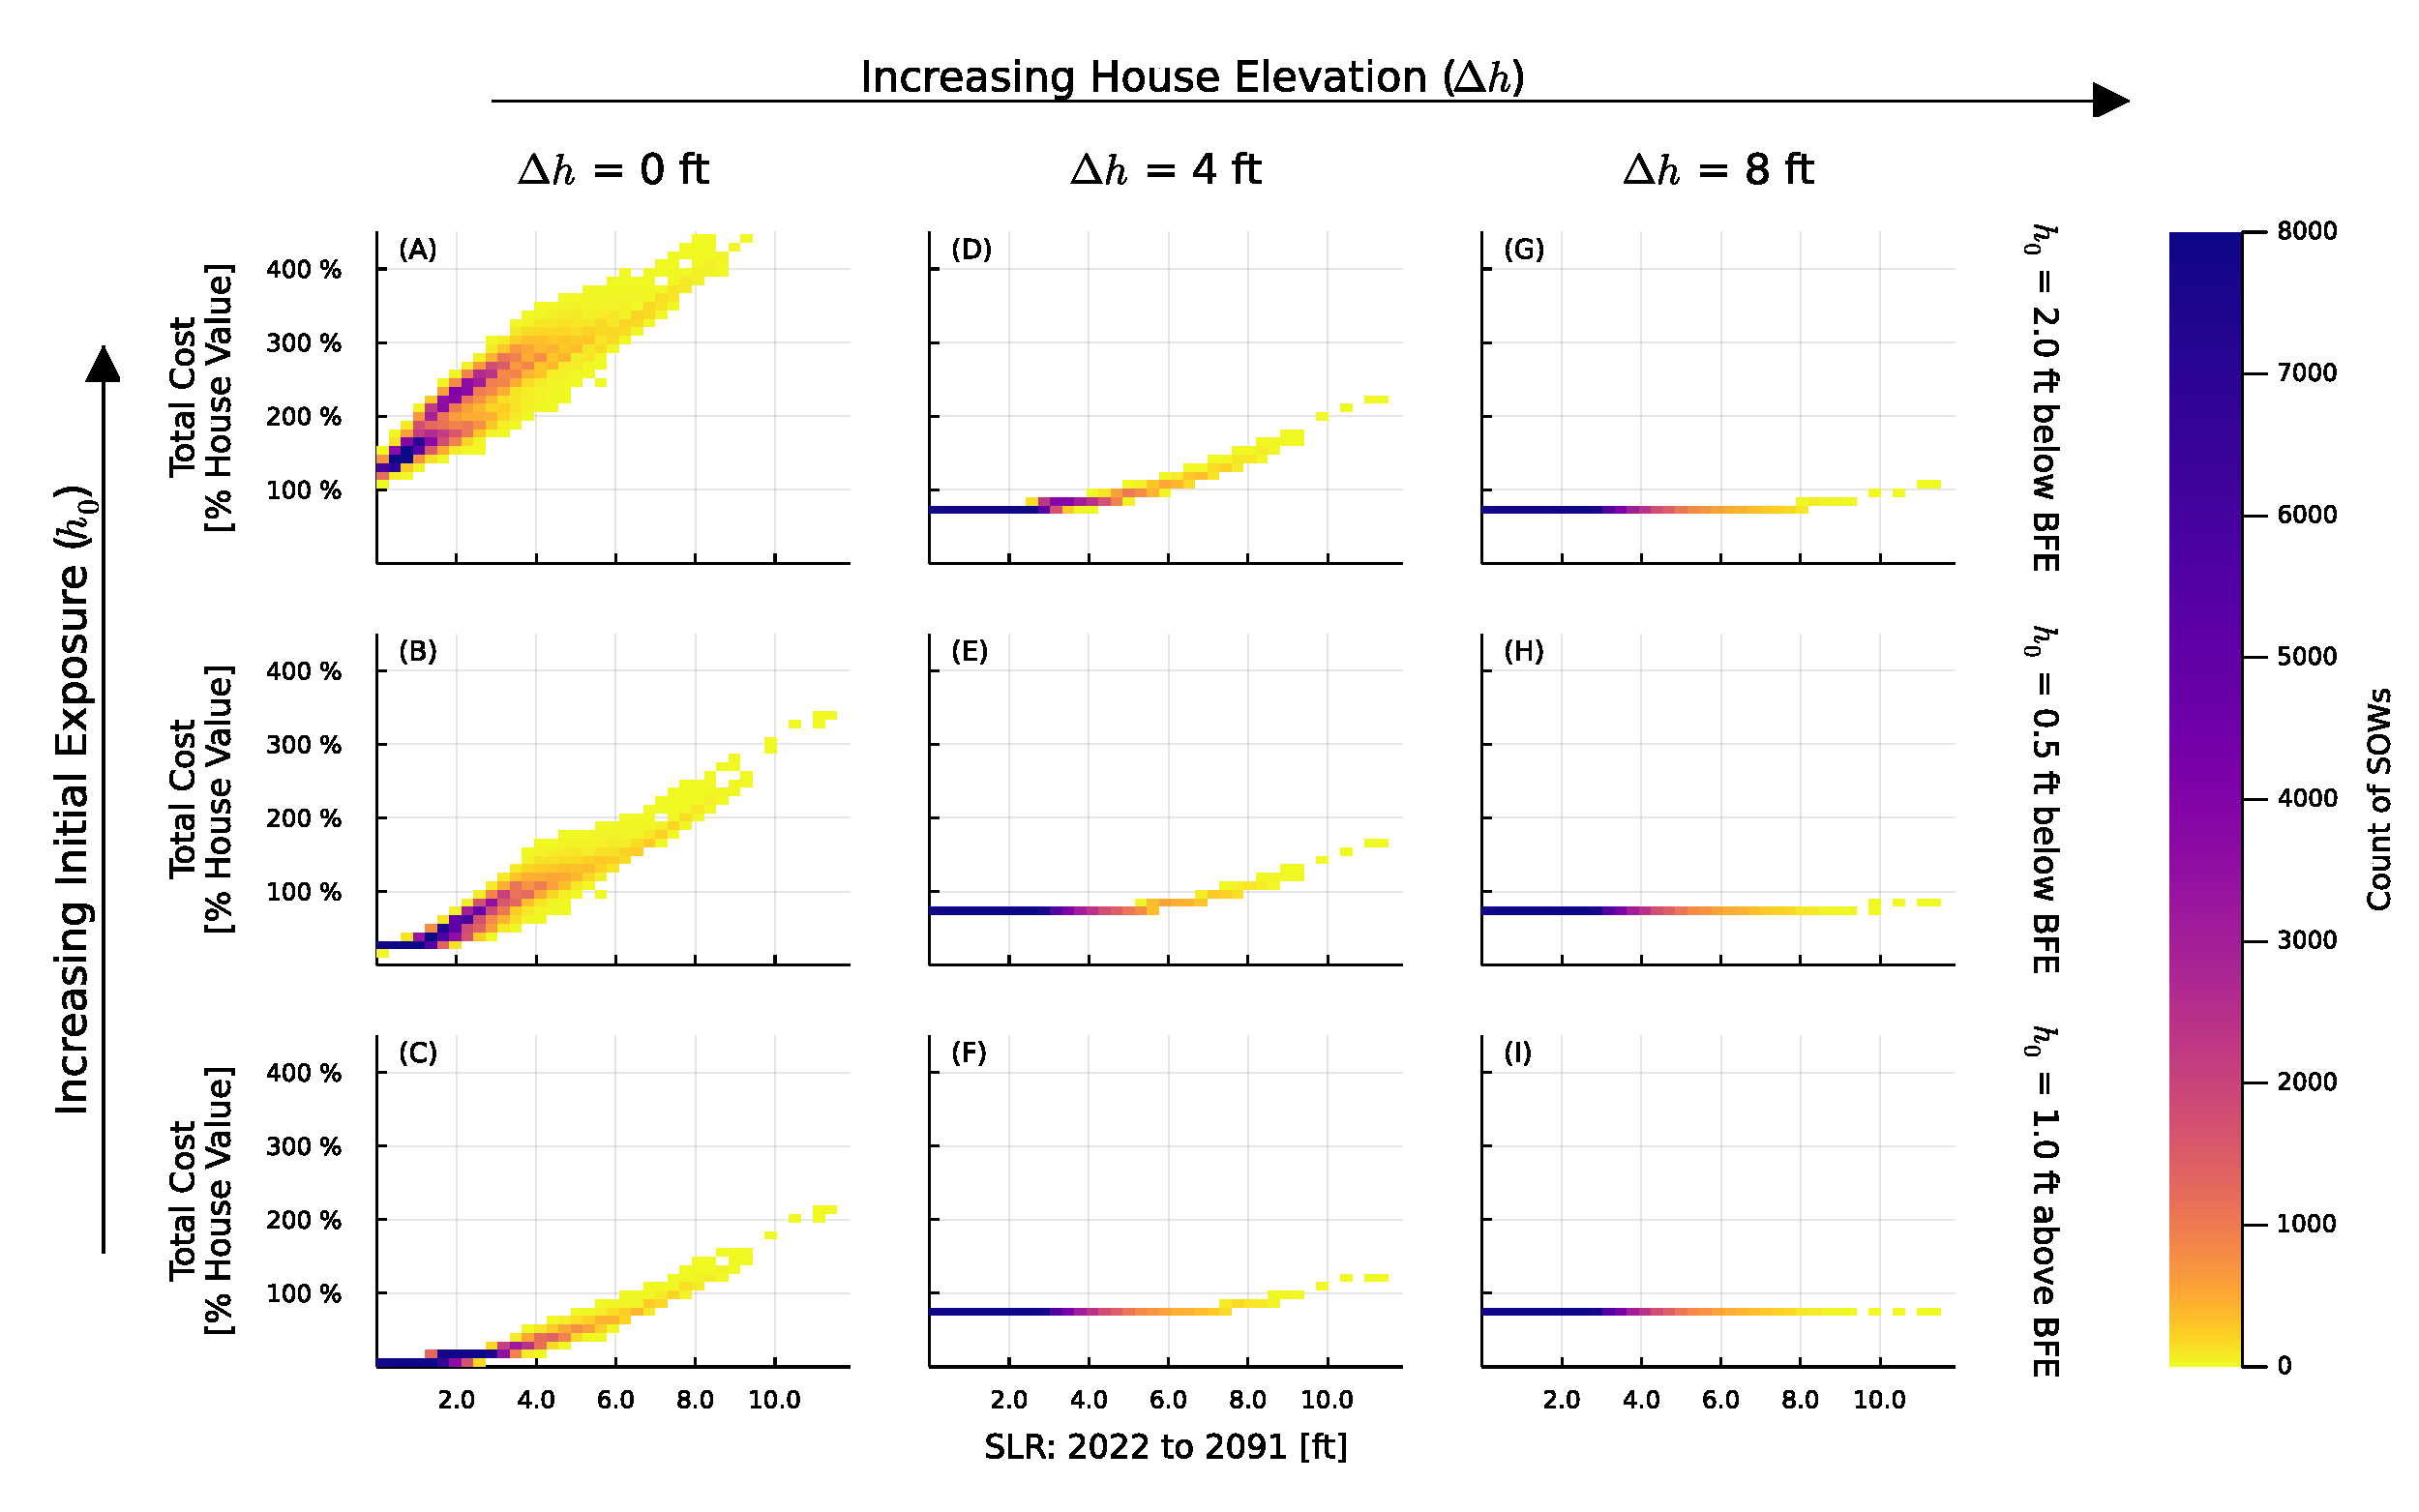
\includegraphics[width=\textwidth]{scenario-map-slr-cost}
    \caption{
        Scenario maps showing the dependence of expected lifetime cost (damages plus up-front cost; eq.XXX) as a function of \gls{slr} in 2100 for several values of $\Delta h$ and $h_0$.
        Colors indicate the density of \glspl{sow}; this data is often presented as a scatterplot (CITE) but we bin to a 2D histogram. % TODO: cite scenario maps
        The lowest-cost outcomes occur when $h_0$ is large, the house is not elevated (no up-front cost), and sea level rise is minimal.
        The highest-cost outcomes arise when the house is not elevated (no up-front cost) and sea level rise is rapid.
        In all cases, elevating the house reduces the variance in total lifetime cost.
        Values are sensitive to model constants; see \cref{tab:uncertainties}.
    }\label{fig:scenario-map-slr-cost}
\end{figure}

\begin{figure}
    \centering
    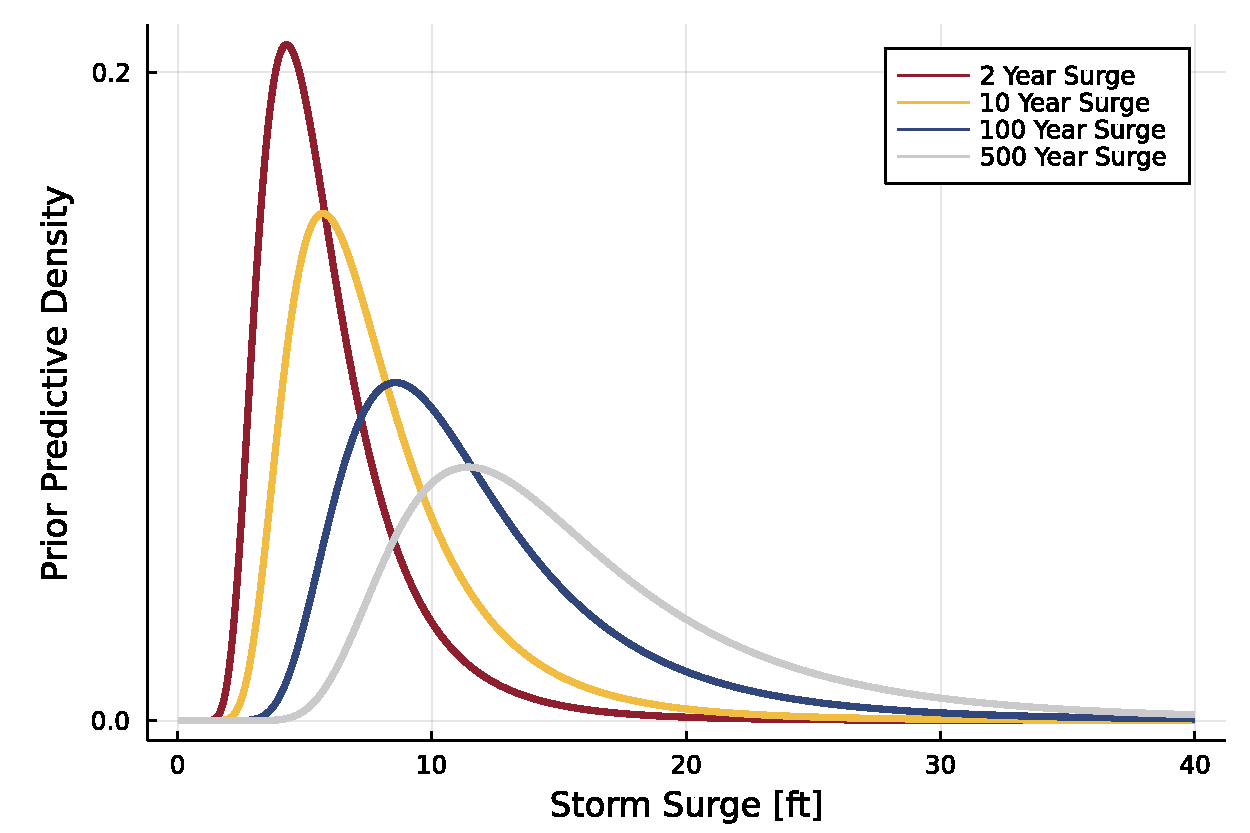
\includegraphics[width=4in]{surge-gev-priors}
    \caption{
        Prior distributions for annual maximum storm surge.
        Rather than apply a prior over model parameters directly, we apply a weakly informative prior over quantiles of the resulting distribution (that is, over a function of the model parameters) following REFERENCE. % TODO: cite
        See ex.~XYQ for details. % TODO: cross-ref equation
        We apply priors over the 2, 10, 100, and 500 year events.
    }\label{fig:surge-gev-priors}
\end{figure}

\begin{figure}
    \centering
    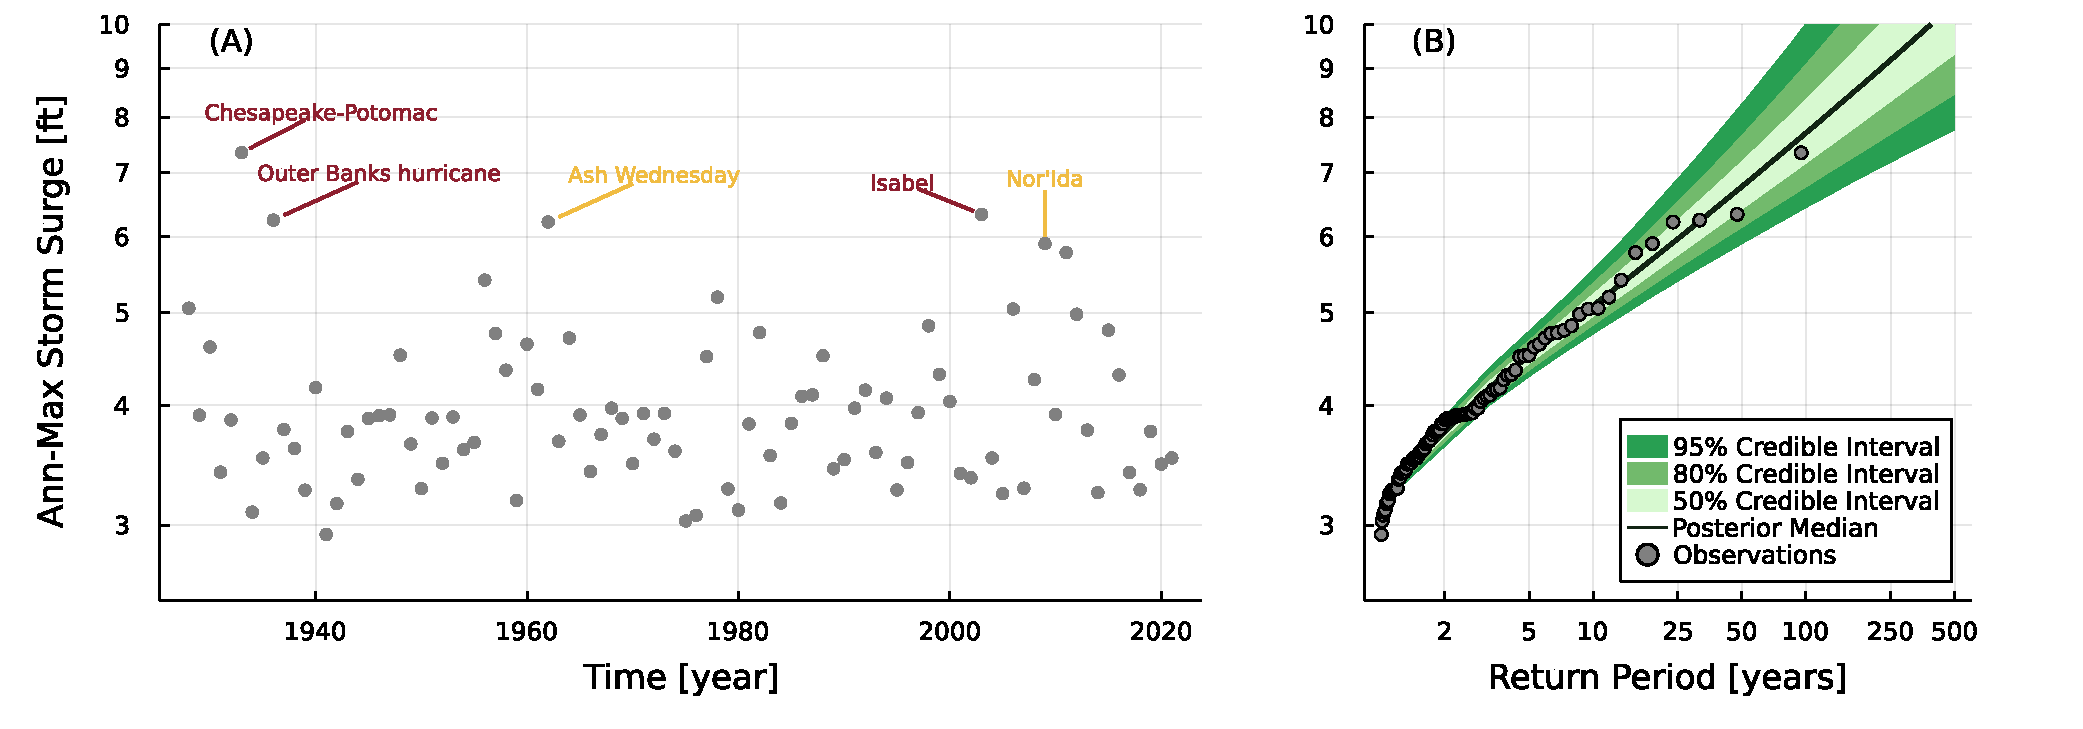
\includegraphics[width=\textwidth]{surge-obs-return}
    \caption{
        Annual maximum storm surges (after subtracting mean sea level) at Sewells Point, VA (CITE SOURCE). % TODO: cite source
        (A):
        Time series of historic storms.
        Blue (green) arrows denote notable tropical cyclones (nor'easters).
        (B):
        Return periods.
        Dots indicate observed values; their $x$-value (``plotting position'') is calculated using the Weibull formula (eq.~\cref{eq:plot-pos}).
        Gray lines show the 50, 80, and 95\% posterior confidence intervals from the Bayesian GEV fit.
    }\label{fig:surge-obs-return}
\end{figure}

\begin{figure}
    \centering
    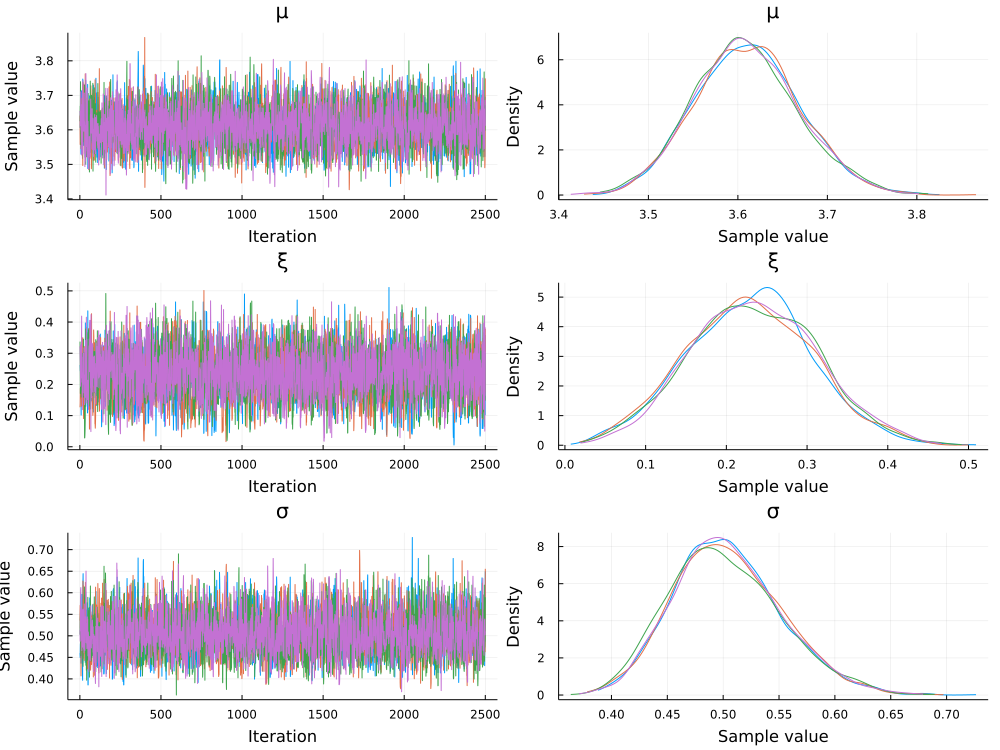
\includegraphics[width=\textwidth]{surge-posterior-chains}
    \caption{
        \Gls{mcmc} plots for posterior draws from the storm surge model.
        We draw \num{10000} samples by running four chains of \num{3500} iterations each and discarding the first \num{1000}.
        The mixing of the chains is consistent with, though does not guarantee, convergence.
    }\label{fig:surge-posterior-chains}
\end{figure}

\begin{figure}
    \centering
    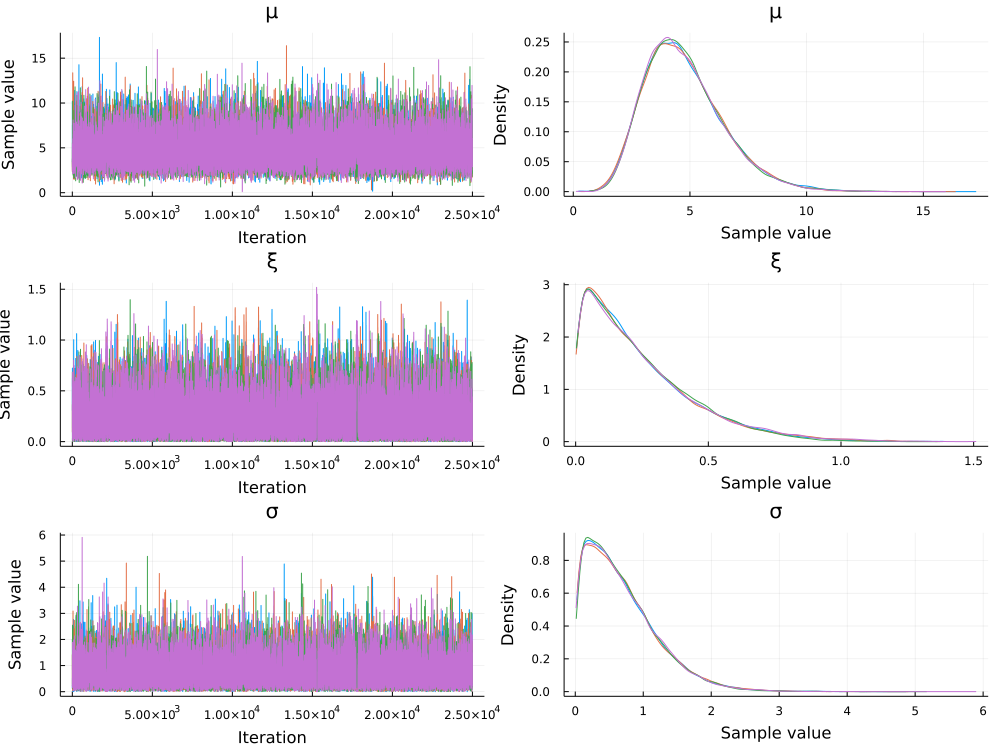
\includegraphics[width=\textwidth]{surge-prior-chains}
    \caption{
        As \cref{fig:surge-posterior-chains} but for draws from the prior distribution.
    }\label{fig:surge-prior-chains}
\end{figure}

\begin{figure}
    \centering
    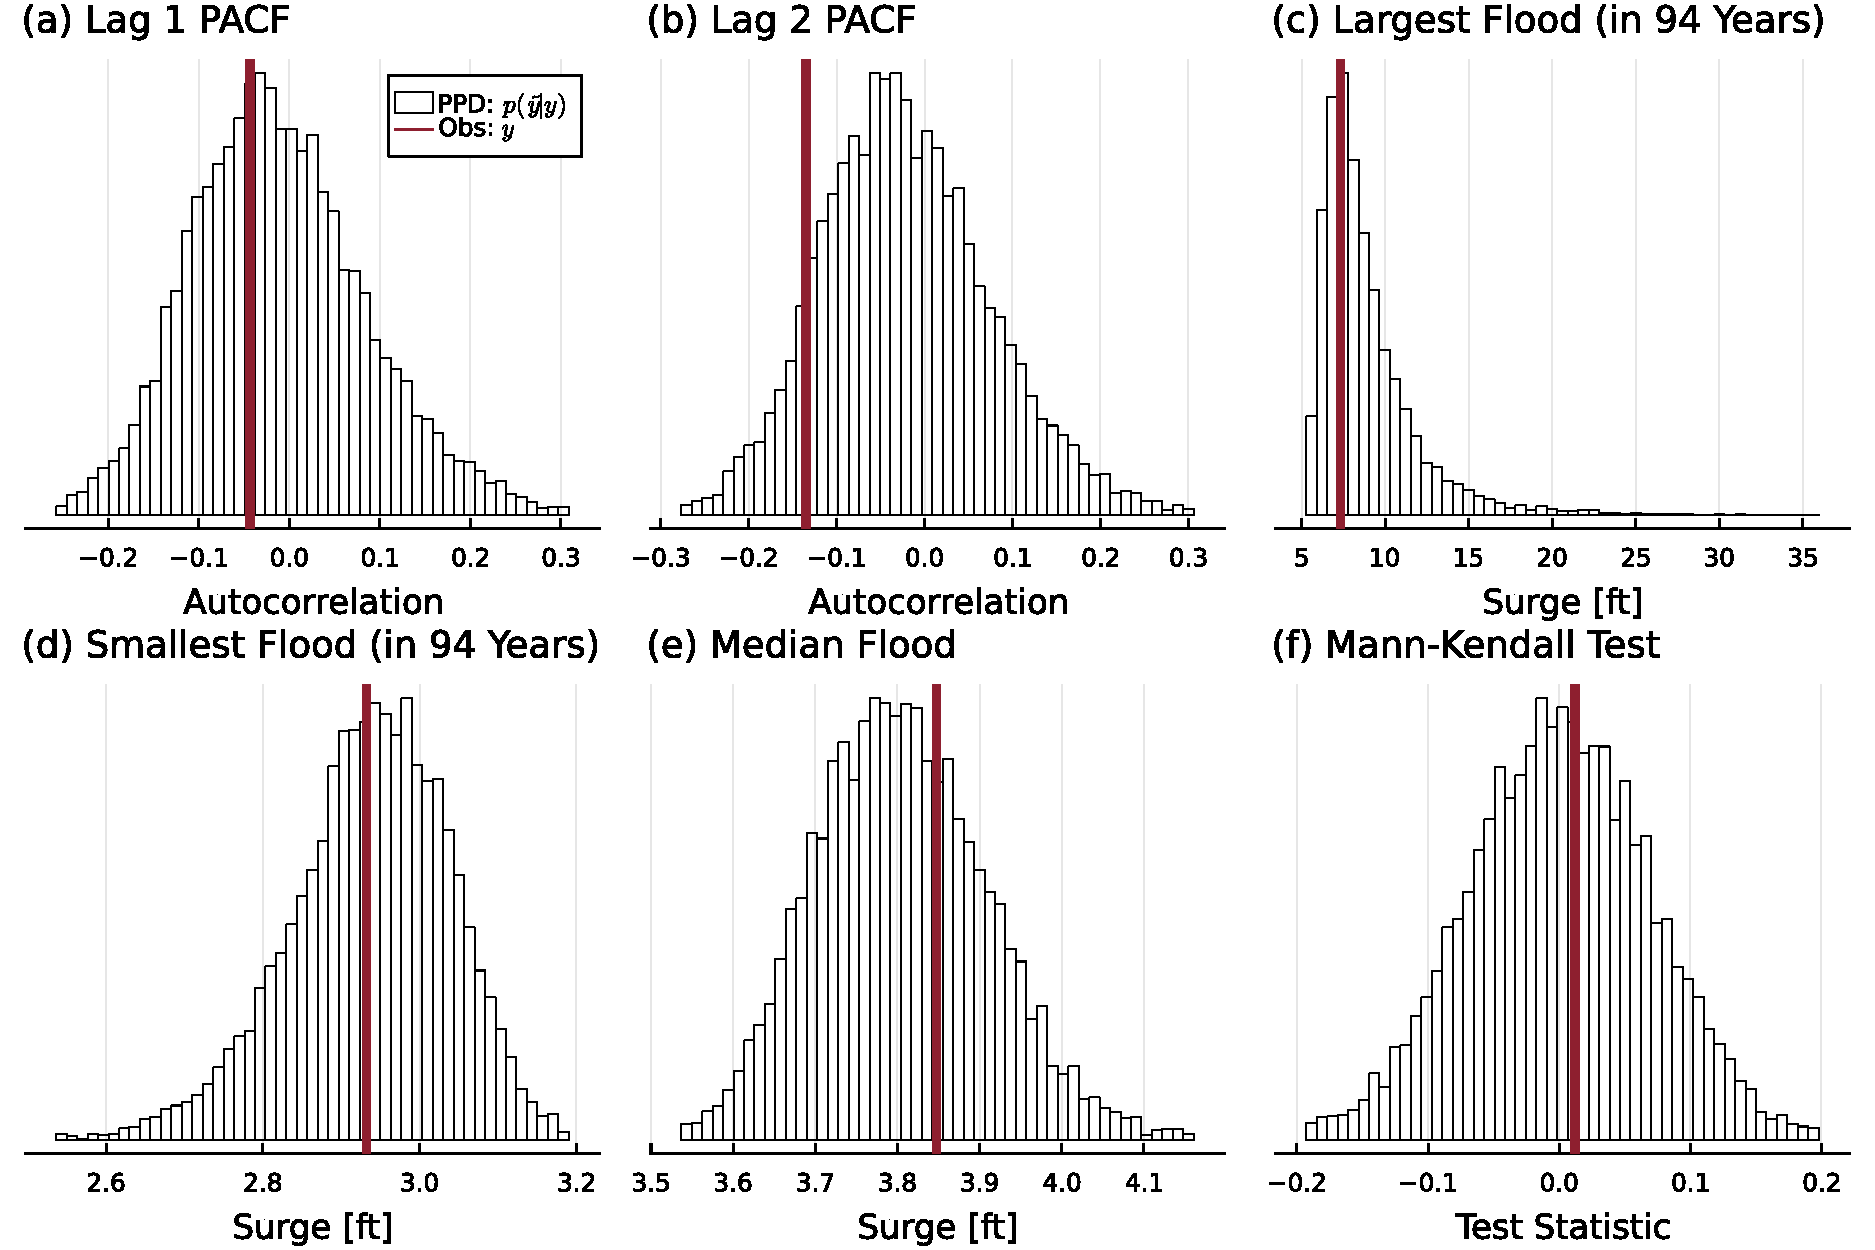
\includegraphics[width=\textwidth]{surge-test-statistics}
    \caption{
        Posterior predictive checks for the stationary GEV storm surge model (section XXX). % TODO: reference section
        Each panel shows a different test statistic: partial autocorrelation at lags 1 and 2; sample maximum; sample minimum; sample median; and Mann-Kendall trend test statistic.
        The histograms show the distribution of each test statistic from the posterior predictive distribution.
        Orange lines show the test statistic's value in the observed data.
        Observed values near the mode of the posterior predictive distribution are consistent with, but do not guarantee, a good fit.
        For further discussion of posterior predictive checks, see Chapter 6 of \citet{Gelman:2014tc}.
    }\label{fig:surge-test-statistics}
\end{figure}

\begin{figure}
    \centering
    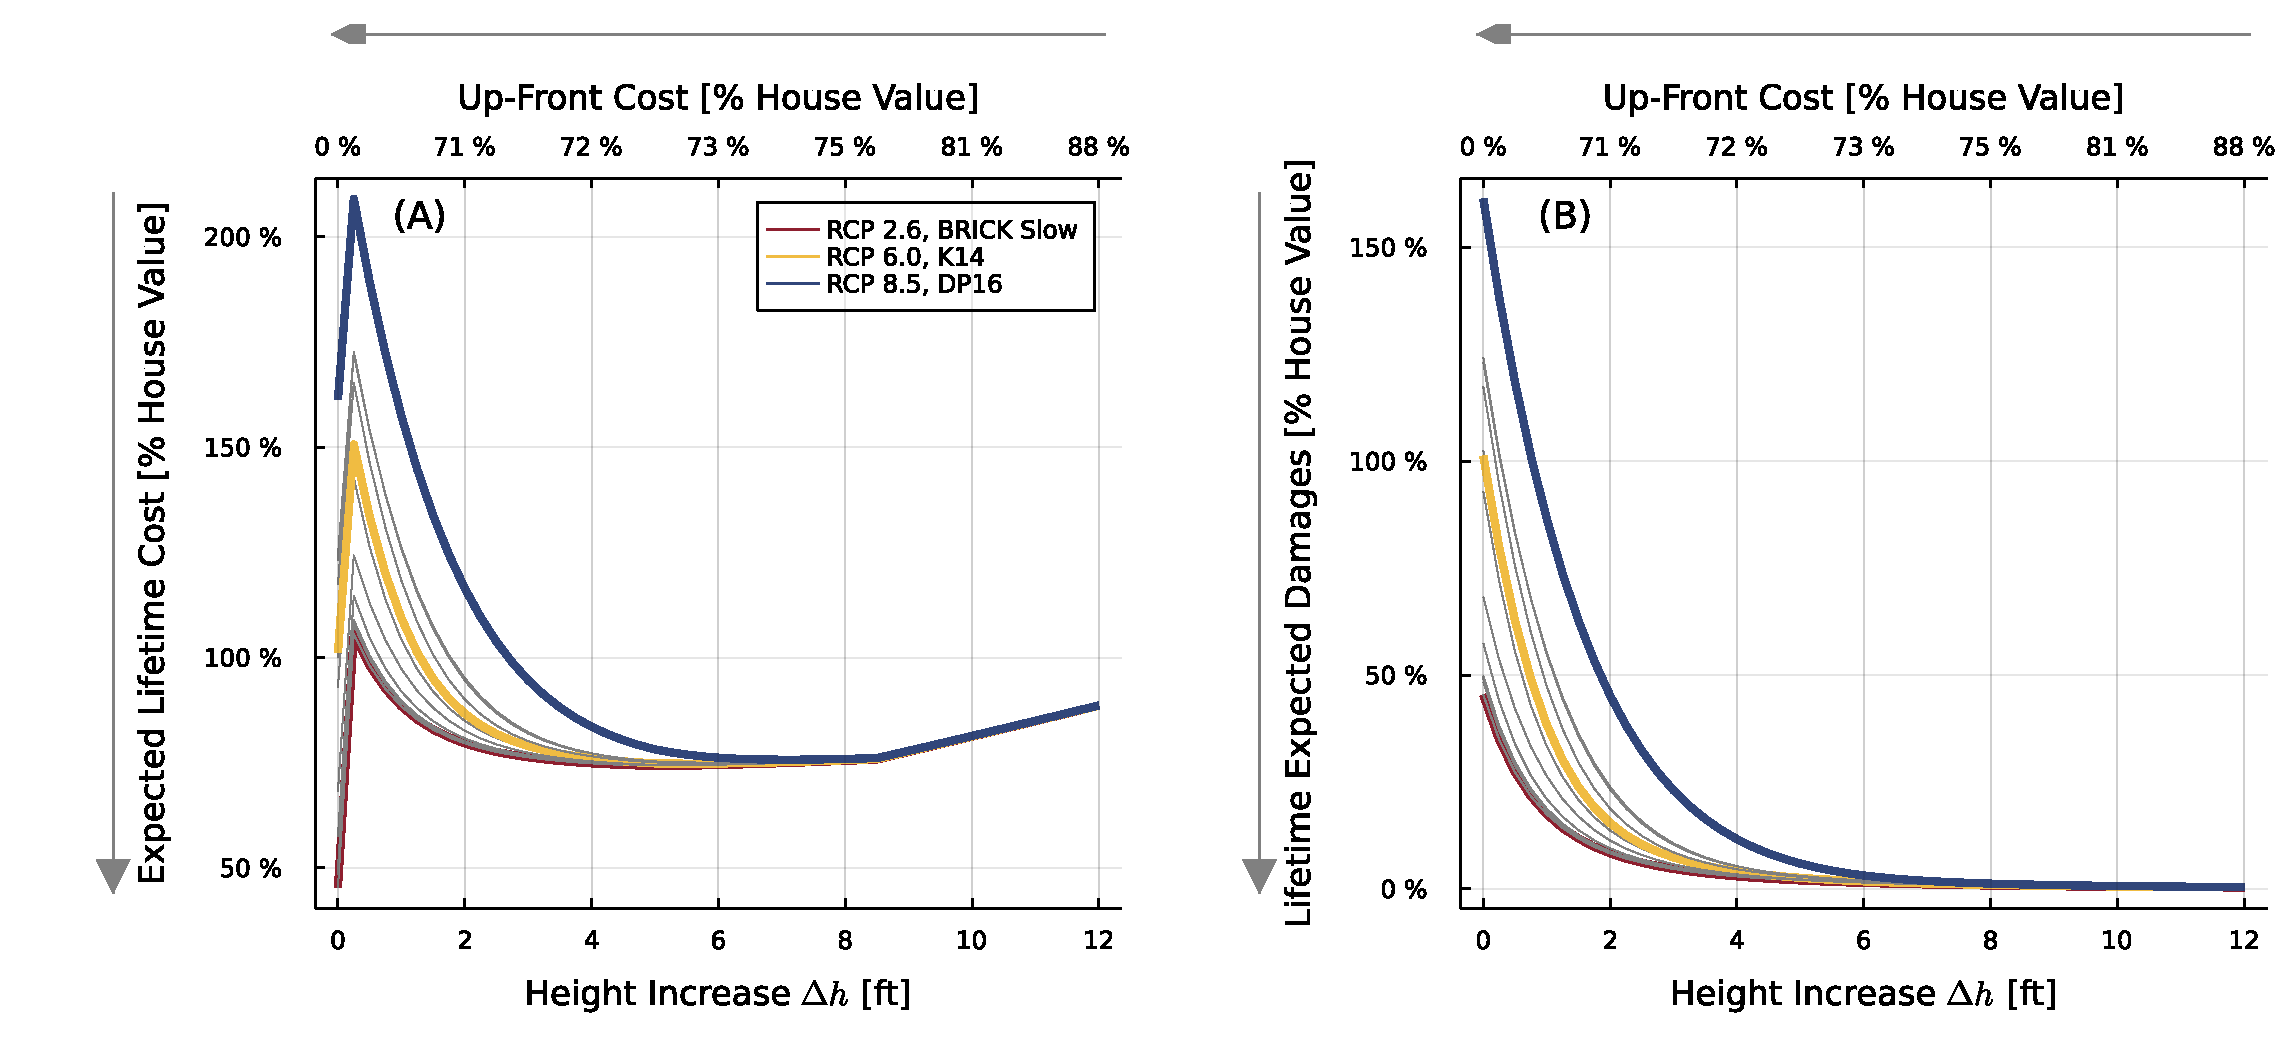
\includegraphics[width=\textwidth]{tradeoffs-by-rcp}
    \caption{
        Each probabilistic model or scenario leads to a different estimate of the Pareto frontier.
        (A): trade-off between up-front cost (which is a monotonic function of height increase) and expected lifetime costs (eq.~XX). % TODO: ref equation
        (B): trade-off between up-front cost and lifetime expected damages (eq.~\ref{eq:led}).
        Light gray lines show estimates for all 16 models (four \gls{rcp} scenarios times four physical parameterizations) considered.
        Colored lines highlight three representative models for emphasis.
    }\label{fig:tradeoffs-by-rcp}
\end{figure}

\begin{figure}
    \centering
    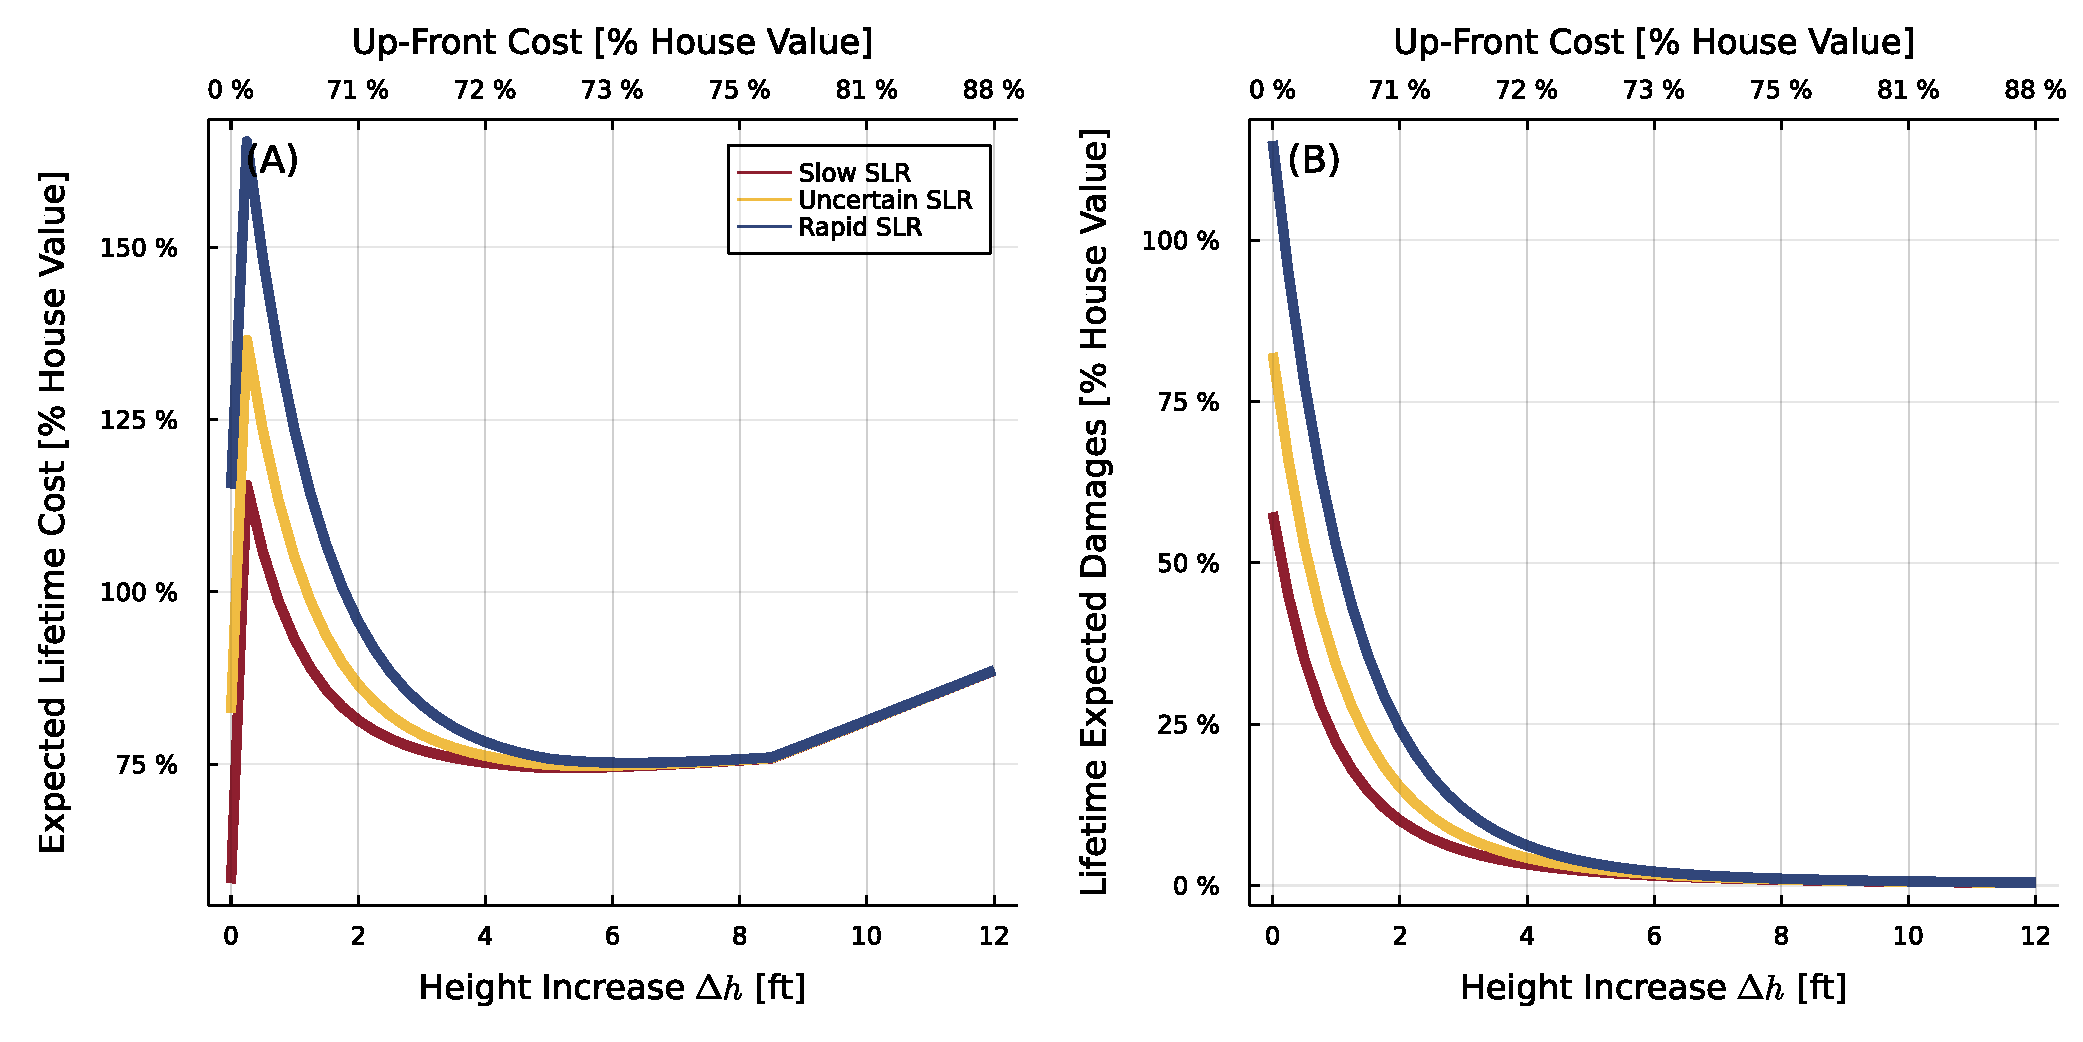
\includegraphics[width=\textwidth]{tradeoffs-by-prior}
    \caption{
        As \cref{fig:tradeoffs-by-rcp}, but Pareto frontiers are shown for the synthesizing Bayesian models.
    }\label{fig:tradeoffs-by-prior}
\end{figure}

\section{Supplemental tables}

\begin{table}[h]
    \centering
    \caption{
        Diagnostic statistics for the \gls{mcmc} sampling for the storm surge posterior draws.
        Statistics include the mean and standard deviation of each parameter, the naive standard error and Monte Carlo standard error (which measure uncertainty in the mean), the effective sample size, $\hat{R}$ diagnostic, and effective samples per second, which describes sampling speed.
        In general, a $\hat{R}$ value close to one is consistent with, though does not guarantee, convergence.
    }\label{tab:surge-posterior-mcmc-diagnostics}
    \begin{tabular}{cccccccc}
\toprule
$\textrm{Parameter}$ & $\textrm{Mean}$ & $\textrm{Stdev.}$ & $\textrm{Naive SE}$ & $\textrm{MCSE}$ & $\textrm{ESS}$ & $\hat{R}$ & $ess_{per\_sec}$\\
\midrule
$\mu$ & $3.610$ & $0.058$ & $0.001$ & $0.001$ & $4819.426$ & $1.000$ & $467.044$\\
$\sigma$ & $0.504$ & $0.049$ & $0.000$ & $0.001$ & $4508.859$ & $1.000$ & $436.947$\\
$\xi$ & $0.231$ & $0.078$ & $0.001$ & $0.001$ & $4729.255$ & $1.001$ & $458.306$\\
\bottomrule
\end{tabular}

\end{table}

\begin{table}[h]
    \centering
    \caption{As \cref{tab:surge-posterior-mcmc-diagnostics} but for draws from the prior distribution.}\label{tab:surge-prior-mcmc-diagnostics}
    \begin{tabular}{ccccccc}
\toprule
$\textrm{Parameter}$ & $\textrm{Mean}$ & $\textrm{Stdev.}$ & $\textrm{Naive SE}$ & $\textrm{MCSE}$ & $\textrm{ESS}$ & $\hat{R}$\\
\midrule
$\mu$ & $4.774$ & $1.702$ & $0.005$ & $0.011$ & $26657.405$ & $1.000$\\
$\xi$ & $0.246$ & $0.215$ & $0.001$ & $0.002$ & $11238.145$ & $1.000$\\
$\sigma$ & $0.682$ & $0.531$ & $0.002$ & $0.004$ & $24720.263$ & $1.000$\\
\bottomrule
\end{tabular}

\end{table}

\end{document}
